\documentclass[12pt,a4paper,oneside]{report}

% =========================================================
% VESIT MINI PROJECT - 2B REPORT TEMPLATE
% Department of Artificial Intelligence and Data Science
% Academic Year: 2026--2027
% =========================================================

\usepackage[utf8]{inputenc}
\usepackage[T1]{fontenc}
\usepackage{graphicx}
\usepackage{amsmath,amssymb}
\usepackage{booktabs}
\usepackage{array}
\usepackage{longtable}
\usepackage{multirow}
\usepackage{float}
\usepackage{caption}
\usepackage{subcaption}
\usepackage{setspace}
\usepackage{geometry}
\usepackage{fancyhdr}
\usepackage{titlesec}
\usepackage{enumitem}
\usepackage{xcolor}
\usepackage{url}
\usepackage[hidelinks]{hyperref}
\usepackage{cite}
\usepackage{listings}
\usepackage{tikz}
\usetikzlibrary{shapes,arrows,positioning}
\usepackage{etoolbox}
\usepackage{pdflscape}

% ---------------------------------------------------------
% Page setup (Standard Academic Margins)
% ---------------------------------------------------------
\geometry{
    a4paper,
    left=1.5in,
    right=1in,
    top=1in,
    bottom=1in
}

\onehalfspacing
\setlength{\parindent}{0.5in}
\setlength{\parskip}{0pt}

% ---------------------------------------------------------
% Project details configuration
% ---------------------------------------------------------
% =========================================================
% PROJECT DETAILS
% VESIT AI&DS Mini Project - 2B
% Academic Year: 2026--2027
% =========================================================

% ---------- Institute ----------
\newcommand{\institutename}{VESIT}
\newcommand{\fullinstitutename}{Vivekanand Education Society's Institute of Technology}
\newcommand{\instituteaffiliation}{(An Autonomous Institute Affiliated to University of Mumbai)}
\newcommand{\instituteaddress}{Hashu Advani Memorial Complex, Collector's Colony, Chembur, Mumbai - 400 074}

\newcommand{\departmentname}{Department of Artificial Intelligence and Data Science}
\newcommand{\shortdepartment}{Department of AI\&DS}

% ---------- Project ----------
\newcommand{\projecttitle}{Impact of Experimental Randomness on ML Model Stability and Reproducibility}
\newcommand{\projectsubtitle}{A Mini Project - 2B Report}
\newcommand{\degreetitle}{Bachelor of Technology in Artificial Intelligence and Data Science}

% ---------- Students (3 Members) ----------
\newcommand{\studentone}{Prem K.K. Bhojwani}
\newcommand{\studentoneprn}{Roll No. 04}

\newcommand{\studenttwo}{Jiya Gurbani}
\newcommand{\studenttwoprn}{Roll No. 15}

\newcommand{\studentthree}{Harsh Dingreja}
\newcommand{\studentthreeprn}{Roll No. 12}

% ---------- Faculty ----------
% Project Guide
\newcommand{\guidename}{Mrs. Bincy Ivin}
\newcommand{\guideDesignation}{Assistant Professor}

% Head of Department
\newcommand{\hodname}{Dr. Anjali Shrikant Yeole}
\newcommand{\hodDesignation}{Head of Department}

% Principal
\newcommand{\principalname}{Dr. J. M. Nair}
\newcommand{\principalDesignation}{Principal}

% ---------- Academic Year ----------
\newcommand{\academicYear}{2026--2027}

% ---------- Logo Locations ----------
\newcommand{\vesitlogo}{figures/VESIT LOGO ICON (1).png}

% ---------- Header Text ----------
\newcommand{\leftheader}{\shortdepartment}
\newcommand{\rightheader}{Mini Project - 2B Report}


% =========================================================
% HEADER AND FOOTER
% =========================================================

\pagestyle{fancy}
\fancyhf{}

% Header
\fancyhead[L]{\small\bfseries \leftheader}
\fancyhead[R]{\small\bfseries \rightheader}

% Header line
\renewcommand{\headrulewidth}{0.5pt}

% Footer
\fancyfoot[C]{\thepage}

% Footer line
\renewcommand{\footrulewidth}{0pt}

% Header/footer spacing
\setlength{\headheight}{16pt}

% Make chapter-opening pages use the same header/footer
\fancypagestyle{plain}{
    \fancyhf{}
    \fancyhead[L]{\small\bfseries \leftheader}
    \fancyhead[R]{\small\bfseries \rightheader}
    \fancyfoot[C]{\thepage}
    \renewcommand{\headrulewidth}{0.5pt}
    \renewcommand{\footrulewidth}{0pt}
}

% ---------------------------------------------------------
% Chapter formatting
% ---------------------------------------------------------
\titleformat{\chapter}[display]
  {\normalfont\bfseries\centering}
  {\chaptername\ \thechapter}
  {10pt}
  {\Large}

\titlespacing*{\chapter}{0pt}{-10pt}{25pt}

% ---------------------------------------------------------
% Captions
% ---------------------------------------------------------
\captionsetup{
    font=small,
    labelfont=bf,
    justification=centering
}

% ---------------------------------------------------------
% Code listing style
% ---------------------------------------------------------
\lstset{
    basicstyle=\ttfamily\footnotesize,
    breaklines=true,
    frame=single,
    numbers=left,
    numberstyle=\tiny,
    showstringspaces=false,
    keywordstyle=\color{blue}\bfseries,
    commentstyle=\color{gray}\itshape,
    stringstyle=\color{teal},
    backgroundcolor=\color{black!2}
}

\begin{document}

% =========================================================
% FRONT MATTER
% =========================================================
\pagenumbering{roman}

\begin{titlepage}
\thispagestyle{empty}

\begin{center}

\vspace*{-0.2cm}

% =========================================================
% INSTITUTE
% =========================================================

{\LARGE\bfseries \fullinstitutename\par}

\vspace{0.3cm}

{\small \instituteaffiliation\par}

\vspace{0.05cm}

{\small \instituteaddress\par}

\vspace{0.35cm}

% =========================================================
% DEPARTMENT
% =========================================================

{\Large\bfseries \departmentname\par}

\vspace{0.35cm}

% =========================================================
% LOGO
% =========================================================

\includegraphics[width=2.8cm]{\vesitlogo}

\vspace{0.4cm}

% =========================================================
% PROJECT TITLE
% =========================================================

{\large A Mini Project - 2B Report on\par}

\vspace{0.2cm}

{\LARGE\bfseries \projecttitle\par}

\vspace{0.4cm}

% =========================================================
% DEGREE
% =========================================================

{\normalsize Submitted in partial fulfillment of the requirements\\for the award of the degree of\\
\textbf{\degreetitle}\par}

\vspace{0.45cm}

% =========================================================
% STUDENTS
% =========================================================

{\normalsize\bfseries Submitted by\par}

\vspace{0.15cm}

\begin{tabular}{ll}
\textbf{\studentone}   & \quad (\studentoneprn) \\
\textbf{\studenttwo}   & \quad (\studenttwoprn) \\
\textbf{\studentthree} & \quad (\studentthreeprn) \\
\end{tabular}

\vspace{0.4cm}

% =========================================================
% GUIDE
% =========================================================

{\normalsize\bfseries Under the Guidance of\par}

\vspace{0.15cm}

{\large\bfseries \guidename\par}
{\normalsize (\guideDesignation)\par}

\vfill

% =========================================================
% ACADEMIC YEAR
% =========================================================

{\large\bfseries Academic Year \academicYear\par}

\vspace{0.1cm}

\end{center}

\end{titlepage}

\chapter*{Certificate}
\addcontentsline{toc}{chapter}{Certificate}

This is to certify that the project entitled \textbf{``\projecttitle''} has been successfully carried out by \textbf{\studentone\ (\studentoneprn)}, \textbf{\studenttwo\ (\studenttwoprn)}, and \textbf{\studentthree\ (\studentthreeprn)} under the guidance of \textbf{\guidename} in partial fulfillment of the requirements for the award of the degree of \textbf{\degreetitle} during the academic year \textbf{\academicYear}.

\vspace{3.5cm}

\begin{table}[H]
\centering
\begin{tabular}{ccc}
\rule{4.5cm}{0.4pt} & \rule{4.5cm}{0.4pt} & \rule{4.5cm}{0.4pt} \\
\textbf{\guidename} & \textbf{\hodname} & \textbf{\principalname} \\
\guideDesignation & \hodDesignation & \principalDesignation \\
\end{tabular}
\end{table}

\vspace{1.5cm}

\begin{table}[H]
\centering
\begin{tabular}{cc}
\rule{5cm}{0.4pt} & \rule{5cm}{0.4pt} \\
\textbf{Internal Examiner} & \textbf{External Examiner} \\
\end{tabular}
\end{table}

\vfill

\noindent Date: \rule{3.5cm}{0.4pt} \hfill Place: Mumbai

\chapter*{Declaration}
\addcontentsline{toc}{chapter}{Declaration}

We hereby declare that the mini project entitled \textbf{``\projecttitle''} is our original work carried out under the guidance of \textbf{\guidename}, \guideDesignation, \departmentname, \fullinstitutename.

The work presented in this report has not been submitted elsewhere for the award of any degree or diploma, except where due reference and acknowledgement have been made in the text.

\vspace{2.5cm}

\begin{table}[H]
\centering
\begin{tabular}{p{7cm} p{7cm}}
\textbf{Name of Student} & \textbf{Signature} \\[1.2cm]
\textbf{\studentone} (\studentoneprn) & \rule{5cm}{0.4pt} \\[1.2cm]
\textbf{\studenttwo} (\studenttwoprn) & \rule{5cm}{0.4pt} \\[1.2cm]
\textbf{\studentthree} (\studentthreeprn) & \rule{5cm}{0.4pt} \\
\end{tabular}
\end{table}

\vfill

\noindent Date: \rule{3.5cm}{0.4pt} \hfill Place: Mumbai

\chapter*{Acknowledgement}
\addcontentsline{toc}{chapter}{Acknowledgement}

We express our deepest sense of gratitude and sincere thanks to our esteemed project guide, \textbf{\guidename}, \guideDesignation, \departmentname, for her continuous encouragement, invaluable guidance, keen interest, and thoughtful suggestions throughout the duration of this mini project.

We would like to convey our heartfelt gratitude to \textbf{\hodname}, \hodDesignation, \departmentname, for providing excellent academic infrastructure and departmental facilities that facilitated the successful completion of this project.

We extend our sincere thanks to \textbf{\principalname}, \principalDesignation, \fullinstitutename, for creating a motivating research and learning environment.

Finally, we express our profound gratitude to our parents, family members, teaching and non-teaching staff, and fellow batchmates for their constant support, encouragement, and cooperation throughout our academic endeavors.

\vspace{2.0cm}

\begin{flushright}
\textbf{\studentone} (\studentoneprn)\\
\textbf{\studenttwo} (\studenttwoprn)\\
\textbf{\studentthree} (\studentthreeprn)
\end{flushright}

\chapter*{Abstract}
\addcontentsline{toc}{chapter}{Abstract}

Machine learning experiments are inherently stochastic: pseudo-random number seeds govern data splitting, model weight initialization, bootstrap sampling, and fold assignment in cross-validation. Without rigorous seed management, repeated runs of the same experiment produce varying outcomes, impairing fair model benchmarking and compromising research reproducibility. This project systematically investigates the impact of experimental randomness on the stability and reproducibility of three representative classification algorithms---Decision Tree, Random Forest, and Linear Support Vector Machine (Linear SVM)---evaluated on the canonical Forest CoverType dataset.

The Forest CoverType dataset, sourced from the UCI Machine Learning Repository via \texttt{scikit-learn}, encompasses 581,012 samples characterized by 54 features (10 continuous cartographic measurements, 4 binary wilderness area indicators, and 40 binary soil-type indicators). To maintain computational tractability while preserving class frequencies, a stratified random subsample of 10,000 records was curated with strict class distribution preservation.

Three empirical investigations were conducted:
\begin{enumerate}
    \item \textbf{Baseline Performance Assessment:} Evaluating classification metrics (Accuracy, Macro-F1, Precision, Recall) across algorithms on a standardized 80/20 stratified train-test split.
    \item \textbf{Split Seed Sensitivity Analysis:} Benchmarking model accuracy variance across five distinct random split seeds (0, 1, 42, 99, 123) under identical hyperparameter configurations.
    \item \textbf{Cross-Validation \& Reproducibility Auditing:} Performing repeated 5-fold stratified cross-validation across three shuffle seeds (11, 22, 33) to measure fold-allocation variance, alongside a bitwise prediction verification verifying deterministic reproducibility across execution cycles.
\end{enumerate}

Empirical results demonstrate that Random Forest achieves superior classification performance (80.80\% baseline accuracy, Macro-F1 0.732) and exhibits the greatest stability with the lowest performance standard deviation across split seeds ($\sigma = 0.58\%$). In contrast, Decision Tree achieves 76.35\% accuracy with higher variance ($\sigma = 0.81\%$), while Linear SVM achieves 71.10\% accuracy ($\sigma = 0.94\%$). The reproducibility audit validates that fixing random seeds guarantees byte-for-byte identical predictions in deterministic environments. This study establishes guidelines for seed transparency, stratified resampling, and robust statistical reporting in applied machine learning.

\vspace{1.0cm}

\noindent \textbf{Keywords:} Machine Learning Reproducibility, Experimental Randomness, Model Stability, Forest CoverType, Random Forest, Decision Tree, Support Vector Machine, Cross-Validation Variance.


\tableofcontents
\listoffigures
\listoftables
\chapter*{List of Abbreviations}
\addcontentsline{toc}{chapter}{List of Abbreviations}

\begin{longtable}{p{3cm} p{11cm}}
\toprule
\textbf{Abbreviation} & \textbf{Full Form} \\
\midrule
\endhead
\bottomrule
\endfoot
\textbf{AI} & Artificial Intelligence \\
\textbf{AIDS / AI\&DS} & Artificial Intelligence and Data Science \\
\textbf{API} & Application Programming Interface \\
\textbf{CART} & Classification and Regression Trees \\
\textbf{CSV} & Comma-Separated Values \\
\textbf{CV} & Cross-Validation \\
\textbf{DT} & Decision Tree \\
\textbf{EDA} & Exploratory Data Analysis \\
\textbf{FN} & False Negative \\
\textbf{FP} & False Positive \\
\textbf{IQR} & Interquartile Range \\
\textbf{ML} & Machine Learning \\
\textbf{PCA} & Principal Component Analysis \\
\textbf{PRNG} & Pseudo-Random Number Generator \\
\textbf{RF} & Random Forest \\
\textbf{SDG} & Sustainable Development Goals \\
\textbf{SVM} & Support Vector Machine \\
\textbf{TN} & True Negative \\
\textbf{TP} & True Positive \\
\textbf{UCI} & University of California, Irvine \\
\textbf{UN} & United Nations \\
\textbf{VESIT} & Vivekanand Education Society's Institute of Technology \\
\bottomrule
\end{longtable}


% =========================================================
% MAIN CONTENT
% =========================================================
\clearpage
\pagenumbering{arabic}

\chapter{Introduction}
\label{ch:introduction}

\section{Background}
\label{sec:background}

Machine learning (ML) has emerged as a cornerstone of modern data-driven computational systems, with impactful applications spanning automated healthcare diagnostics, algorithmic financial risk assessment, natural language comprehension, autonomous navigation, and geospatial ecological monitoring. As reliance on machine learning expands across high-stakes domains, the requirements for experimental reliability, reproducibility, and rigorous methodological standards have become paramount.

A fundamental yet frequently overlooked facet of machine learning experimentation is the profound influence of \textit{stochasticity} (experimental randomness). In conventional ML pipelines, pseudo-random number generators (PRNGs) govern numerous critical operational phases:
\begin{enumerate}[label=(\roman*)]
    \item \textbf{Data Splitting:} The random partitioning of observational samples into training, validation, and testing partitions;
    \item \textbf{Parameter Initialization:} The stochastic initialization of feature splits, internal thresholds, or numerical solver weights;
    \item \textbf{Resampling and Subspacing:} The stochastic selection of bootstrap samples and candidate feature subsets during ensemble generation (e.g., in Random Forests);
    \item \textbf{Cross-Validation Fold Assignment:} The random allocation of data records across $k$ cross-validation partitions.
\end{enumerate}

Each of these stochastic factors can induce variations in reported performance metrics---sometimes by several percentage points---without any modification to the underlying model architecture, hyperparameter configuration, or raw dataset. 

The Forest CoverType benchmark dataset, originally collected by the US Geological Survey (USGS) and US Forest Service (USFS) and made available via the UCI Machine Learning Repository \cite{blackard1999comparative}, provides an ideal benchmark for examining these phenomena. Encompassing 581,012 observations characterized by 54 cartographic and geological features across seven distinct forest cover categories, the dataset features substantial class imbalance, continuous spatial gradients, and sparse binary encodings. Investigating how experimental randomness manifests across diverse model families on this dataset provides direct insight into model sensitivity, algorithmic robustness, and scientific reproducibility.

\section{Problem Statement}
\label{sec:problem_statement}

In machine learning research and engineering practice, reported model performance is frequently derived from a single arbitrary train-test partition using an unrecorded or default random seed (such as \texttt{random\_state=42} or \texttt{None}). Consequently:
\begin{itemize}
    \item \textbf{Lack of Seed Reporting:} Benchmark performance comparisons often fail to state whether observed gains stem from algorithmic superiority or fortunate seed configurations;
    \item \textbf{Single-Split Volatility:} A single partition provides a high-variance point estimate that fails to reflect model stability under distribution shifts;
    \item \textbf{Differential Sensitivity:} Distinct machine learning paradigms (e.g., decision trees, ensemble bagging, and maximum-margin hyperplanes) exhibit drastically different vulnerabilities to stochastic perturbations;
    \item \textbf{Scientific Non-Reproducibility:} Inability to replicate reported empirical results due to unseeded data shuffles, platform-dependent floating-point rounding, or undocumented preprocessing order.
\end{itemize}

This project addresses the central problem: \textit{How significantly does experimental randomness (data partitioning seeds, fold allocation, and sample size) influence classification performance, metric stability, and reproducibility across distinct machine learning algorithms?}

\section{Motivation}
\label{sec:motivation}

The motivation for this investigation stems from three core imperatives:
\begin{enumerate}
    \item \textbf{The Machine Learning Reproducibility Crisis:} Prominent machine learning literature (e.g., Bouthillier et al. \cite{bouthillier2019unreproducible}, Dodge et al. \cite{dodge2020fine}, Lucic et al. \cite{lucic2018gans}) has demonstrated that seed variance can obscure genuine algorithmic improvements, leading to false claims of algorithmic superiority.
    \item \textbf{Critical Environmental Applications:} In ecological management, such as forest resource inventory and wildfire risk mitigation, unreliable model classifications can lead to detrimental conservation policies and ineffective resource allocation.
    \item \textbf{Sound Educational \& Industry Standards:} Demonstrating the critical necessity of standardized cross-validation, explicit seed logging, and stratified resampling provides essential practical discipline for machine learning students and practitioners.
\end{enumerate}

\section{Objectives}
\label{sec:objectives}

The primary objectives of this mini project are formulated as follows:
\begin{enumerate}
    \item \textbf{Dataset Curation and Exploratory Data Analysis (EDA):} Ingest the 581,012-sample Forest CoverType dataset via \texttt{scikit-learn}, perform comprehensive univariate, bivariate, and correlation analyses, and construct a stratified subsample of 10,000 samples to enable rigorous multi-seed experimental iterations.
    \item \textbf{Baseline Algorithmic Evaluation:} Implement, train, and evaluate three distinct classification paradigms---Decision Tree (CART), Random Forest, and Linear Support Vector Machine (Linear SVM)---on a standardized 80/20 stratified split, recording Accuracy, Macro-Precision, Macro-Recall, and Macro-F1 scores.
    \item \textbf{Split Seed Sensitivity Quantification:} Train each algorithm across five distinct pseudo-random data split seeds ($S \in \{0, 1, 42, 99, 123\}$) while keeping hyperparameters constant, computing mean performance and sample standard deviation ($\sigma$) to quantify stability.
    \item \textbf{Cross-Validation Variability Assessment:} Execute 5-fold stratified cross-validation across three distinct shuffle seeds ($S_{\text{CV}} \in \{11, 22, 33\}$) to benchmark fold-assignment stability against single-split variance.
    \item \textbf{Deterministic Reproducibility Verification:} Conduct back-to-back replicated training and inference runs with fixed seeds to verify bitwise identical prediction output.
    \item \textbf{Empirical Guidelines Formulation:} Synthesize actionable best practices for seed transparency, stratified resampling, and robust experimental reporting.
\end{enumerate}

\section{Scope of the Project}
\label{sec:scope}

The project scope encompasses:
\begin{itemize}
    \item Three foundational supervised classification architectures: single tree (\texttt{DecisionTreeClassifier}), bagging ensemble (\texttt{RandomForestClassifier}), and linear margin classifier (\texttt{LinearSVC}).
    \item The canonical Forest CoverType multiclass dataset (7 ecological classes, 54 attributes).
    \item A stratified 10,000-sample representative subset ensuring identical class proportions to the full population while enabling fast, multi-iteration experimentation.
    \item Robust preprocessing protocols, specifically standard feature scaling applied strictly to continuous variables without data leakage.
    \item Exhaustive evaluation using overall Accuracy, macro-averaged Precision, Recall, and F1-score, alongside comprehensive per-class classification reports.
\end{itemize}

\textit{Exclusions:} Hyperparameter grid searches, deep neural networks, and non-tabular synthetic data generation lie beyond the designated scope of this mini project.

\section{Contributions}
\label{sec:contributions}

The key contributions of this research study are:
\begin{itemize}
    \item \textbf{Controlled Experimental Framework:} Formulated an isolated, modular experimental pipeline in Python that isolates seed stochasticity from hyperparameter variance.
    \item \textbf{Empirical Stability Hierarchy:} Demonstrated that Random Forest exhibits the lowest variance ($\sigma = 0.58\%$) across split seeds, outperforming Decision Trees ($\sigma = 0.81\%$) and Linear SVM ($\sigma = 0.94\%$).
    \item \textbf{Cross-Validation Variance Proof:} Confirmed that stratified 5-fold cross-validation substantially reduces estimator variance compared to single arbitrary holdout splits.
    \item \textbf{Reproducibility Guarantee:} Proved that deterministic seed management in \texttt{scikit-learn} achieves complete bitwise reproducibility across independent execution instances.
\end{itemize}

\section{Organization of the Report}
\label{sec:organization}

The remainder of this report is structured as follows:
\begin{itemize}
    \item \textbf{Chapter \ref{ch:literature_review} (Literature Review):} Reviews seminal literature on machine learning reproducibility, random seed sensitivity, and algorithmic benchmarks on the Forest CoverType dataset.
    \item \textbf{Chapter \ref{ch:methodology} (Proposed Methodology):} Details the mathematical formulations, dataset properties, stratified subsampling strategy, preprocessing protocols, and evaluation metrics.
    \item \textbf{Chapter \ref{ch:system_design} (System Design):} Outlines the end-to-end system architecture, workflow pipelines, and data flow representations.
    \item \textbf{Chapter \ref{ch:implementation} (Implementation):} Describes the software environment, library dependencies, implementation scripts, and modular code architecture.
    \item \textbf{Chapter \ref{ch:results} (Results and Discussion):} Presents tabular benchmarks, visual plots, seed variance distributions, and comparative analyses.
    \item \textbf{Chapter \ref{ch:conclusion} (Conclusion and Future Scope):} Summarizes the primary findings, outlines methodological limitations, and charts prospective research extensions.
    \item \textbf{Appendix \& Logbook:} Contains United Nations Sustainable Development Goals (SDG) alignment, 12-week project review logbook, and comprehensive graphical visual results.
\end{itemize}

\chapter{Literature Review}
\label{ch:literature_review}

\section{Introduction}
\label{sec:lit_intro}

Reproducibility and robustness constitute foundational pillars of the scientific method. In computational disciplines such as machine learning and artificial intelligence, an experiment is termed reproducible if an independent researcher, using identical raw data and source code under matching computational conditions, obtains identical or statistically indistinguishable results. However, modern empirical machine learning literature frequently exhibits what prominent researchers refer to as a \textit{reproducibility crisis}. Studies frequently report minor performance margins (e.g., $0.5\%$--$1.5\%$ gains) derived from a single experimental iteration without confidence intervals, statistical hypothesis tests, or explicit seed tracking.

This chapter systematically examines prior literature across three core thematic domains: (i) foundational classification studies on the Forest CoverType benchmark, (ii) algorithmic principles of the benchmarked classifiers, and (iii) recent scholarly investigations into experimental randomness, seed variance, and machine learning stability.

\section{Existing Systems}
\label{sec:existing_systems}

Traditional machine learning benchmarking systems and automated modeling pipelines historically focused almost exclusively on point performance metrics, such as raw classification accuracy or area under the ROC curve (ROC-AUC). Standard practice commonly involves:
\begin{enumerate}
    \item Splitting data using arbitrary default seeds (such as \texttt{random\_state=42} or \texttt{None});
    \item Executing a single training-testing cycle;
    \item Selecting the model exhibiting the highest point accuracy;
    \item Publishing or deploying the model without quantifying stability or variance across alternative partitions.
\end{enumerate}

Such conventional approaches suffer from substantial limitations. When test sets are small or feature distributions are heterogeneous, performance estimates derived from a single partition exhibit high variance. Furthermore, without controlling seed stochasticity, what appears to be an algorithmic advancement may simply be the consequence of a favorable data partition.

\section{Review of Research Papers}
\label{sec:review_papers}

The academic literature relevant to this study is reviewed systematically below:

\paragraph{Forest CoverType Benchmarking:}
The landmark study by Blackard and Dean (1999) \cite{blackard1999comparative} introduced the Forest CoverType dataset to evaluate the comparative predictive capabilities of artificial neural networks (ANNs) versus multivariate discriminant analysis (MDA). Their findings demonstrated that non-linear architectures outperformed linear classifiers, with ANNs achieving approximately 70.5\% accuracy compared to 58.4\% for MDA. Their work established cartographic and elevation variables as dominant predictors of forest species distribution, while highlighting the difficulty of handling severe class imbalance across the seven categories.

\paragraph{Algorithmic Foundations of Classifiers:}
Quinlan (1986) \cite{quinlan1986induction} formulated the foundational principles of top-down induction of decision trees (TDIDT), culminating in the CART and C4.5 algorithms. Decision trees partition feature space orthogonal to feature axes using impurity criteria such as Gini impurity or Shannon entropy. While highly interpretable, individual decision trees are notoriously high-variance estimators: minor perturbations in training instances near split boundaries can cascade into entirely distinct tree structures.

To mitigate tree instability, Breiman (2001) \cite{breiman2001random} introduced the Random Forest algorithm. By combining bootstrap aggregating (bagging) with random feature subspacing at each candidate split, Random Forest dramatically reduces estimator variance without inflating bias. Breiman proved mathematically that as the number of ensemble trees grows, the generalization error converges to a bounded limit, rendering the ensemble remarkably resilient to localized noise.

Cortes and Vapnik (1995) \cite{cortes1995support} introduced Support Vector Networks (SVM), which formulate classification as a convex quadratic optimization problem aimed at maximizing the geometric margin between hyperplanes separating distinct classes. For high-dimensional datasets with extensive binary indicators, linear SVMs offer strong theoretical guarantees against overfitting, though their sensitivity to feature magnitude necessitates careful feature normalization.

Pedregosa et al. (2011) \cite{pedregosa2011scikit} developed \texttt{scikit-learn}, an open-source machine learning library in Python providing unified APIs for classification, regression, and clustering. The library standardizes pseudo-random number generator management via explicit \texttt{random\_state} parameters across estimators and data-splitting routines, establishing the foundational software substrate for modern reproducible ML research.

\paragraph{Empirical Studies on Randomness and Reproducibility:}
In recent years, the machine learning community has increasingly scrutinized the role of pseudo-random seeds. Bouthillier et al. (2019) \cite{bouthillier2019unreproducible} conducted an extensive empirical study on the sources of variance in deep learning, demonstrating that data order and random initialization account for substantial performance dispersion that often exceeds reported state-of-the-art margins. They argued that reporting distributions across multiple seeds is essential for scientific validity.

Dodge et al. (2020) \cite{dodge2020fine} demonstrated that in fine-tuning large language models, varying solely the random seed while keeping all hyperparameters identical yielded dramatic differences in validation accuracy, with some seeds failing to converge altogether. They advocated for explicit seed reporting and multi-seed averaging as mandatory publication standards.

Lucic et al. (2018) \cite{lucic2018gans} conducted a large-scale computational study on generative adversarial networks (GANs), demonstrating that algorithmic improvements reported across multiple publications were statistically indistinguishable once seed variance and hyperparameter budgets were strictly controlled.

\begin{table}[H]
\centering
\small
\caption{Comprehensive Summary of Reviewed Research Literature}
\label{tab:literature_summary}
\begin{tabular}{p{2.2cm} p{2.8cm} p{3.2cm} p{3.2cm} p{2.2cm}}
\toprule
\textbf{Author(s) \& Year} & \textbf{Title / Domain} & \textbf{Methodology} & \textbf{Key Findings} & \textbf{Relevance to Project} \\
\midrule
Blackard \& Dean (1999) \cite{blackard1999comparative} & Forest CoverType Prediction & Compared ANNs and Discriminant Analysis on 581k records & ANNs (70.5\%) outperformed MDA (58.4\%); cartography is predictive & Dataset source and baseline domain benchmark \\
\midrule
Breiman (2001) \cite{breiman2001random} & Random Forests & Bagging plus random subspace feature selection & Variance reduction through de-correlated trees & Theoretical basis for RF stability \\
\midrule
Pedregosa et al. (2011) \cite{pedregosa2011scikit} & Scikit-learn ML in Python & Modular Python ML framework with explicit PRNG & Standardized estimator API and seed control & Implementation framework \\
\midrule
Bouthillier et al. (2019) \cite{bouthillier2019unreproducible} & Unreproducible Research & Empirical decomposition of ML variance sources & Seed variance often exceeds model improvement margins & Motivation for split seed sensitivity testing \\
\midrule
Dodge et al. (2020) \cite{dodge2020fine} & Seed Variance in Deep Learning & Fine-tuning models across different random seeds & Multi-seed evaluation is mandatory for valid benchmarking & Methodological foundation for seed experiments \\
\midrule
Lucic et al. (2018) \cite{lucic2018gans} & Algorithmic Comparison Rigor & Evaluated generative models under controlled budgets & State-of-the-art gains disappeared under seed control & Validates necessity of seed benchmarking \\
\midrule
Cortes \& Vapnik (1995) \cite{cortes1995support} & Support-Vector Networks & Maximum margin hyperplane with slack variables & Convex optimization yields global minimum & Linear SVM baseline model \\
\midrule
Quinlan (1986) \cite{quinlan1986induction} & Induction of Decision Trees & Greedy recursive feature splitting via impurity & High interpretability but high structural variance & Decision Tree baseline model \\
\bottomrule
\end{tabular}
\end{table}

\section{Research Gap}
\label{sec:research_gap}

While theoretical properties of ensemble methods and the sensitivity of deep learning architectures have received substantial attention, several critical empirical research gaps remain:
\begin{enumerate}
    \item \textbf{Tabular Benchmark Focus:} Most recent reproducibility literature concentrates heavily on deep learning and NLP architectures, leaving tabular multi-class classification underexplored regarding multi-seed sensitivity.
    \item \textbf{Direct Cross-Paradigm Sensitivity Comparison:} Few empirical studies benchmark the exact variance degradation profiles of tree-based versus linear-margin models side-by-side on identical high-dimensional tabular data.
    \item \textbf{Practical Seed Audit Guidelines:} Practical frameworks for verifying bitwise reproducibility and quantifying seed-induced variance in academic project workflows remain underdeveloped.
\end{enumerate}

\section{Summary}
\label{sec:lit_summary}

The reviewed literature establishes that experimental randomness is a non-trivial, deterministic factor in machine learning outcomes. While ensemble methods like Random Forest are theoretically designed to minimize variance, quantifying their practical stability against single-tree and linear models on complex real-world data like Forest CoverType provides critical empirical validation. The subsequent chapter outlines our proposed methodology to address these questions.

\chapter{Proposed Methodology}
\label{ch:methodology}

\section{Overview}
\label{sec:method_overview}

This chapter details the proposed experimental methodology designed to rigorously evaluate and quantify the impact of experimental randomness on machine learning models. The framework isolates random seed variations while preserving consistent feature representations, algorithmic hyperparameters, and evaluation protocols. By comparing Decision Tree, Random Forest, and Linear Support Vector Machine on the Forest CoverType dataset, the methodology evaluates both point classification efficacy and statistical distribution stability.

\section{System Requirements}
\label{sec:sys_req}

To ensure complete computational reproducibility, the hardware and software environments were strictly standardized as detailed in Table \ref{tab:system_requirements}.

\begin{table}[H]
\centering
\caption{Computational Environment and System Specifications}
\label{tab:system_requirements}
\begin{tabular}{p{4cm} p{10cm}}
\toprule
\textbf{Component} & \textbf{Specification / Value} \\
\midrule
Operating Environment & Google Colaboratory / Linux x86\_64 (Ubuntu 22.04 LTS) \\
Host Architecture & Intel Xeon CPU @ 2.20GHz (2 vCPUs) \\
Physical Memory (RAM) & 12.67 GB Available System RAM \\
Disk Storage & 107.72 GB Available Virtual Disk \\
Programming Language & Python 3.10.12 \\
Core Libraries & Scikit-learn (1.2.2+), NumPy (1.24.3+), Pandas (2.0.3+), Matplotlib (3.7.1+), Seaborn (0.12.2+) \\
Development Interface & Jupyter Notebook (.ipynb) \\
\bottomrule
\end{tabular}
\end{table}

\section{Proposed Approach}
\label{sec:proposed_approach}

The experimental architecture is structured into sequential investigatory phases:
\begin{enumerate}
    \item \textbf{Data Ingestion \& Exploratory Analysis:} Load the 581,012-sample dataset, audit class distributions, verify absence of missing values, and construct an exact 10,000-sample stratified subset.
    \item \textbf{Phase 1 --- Baseline Modeling:} Split data into 80\% training and 20\% testing sets using a fixed baseline seed ($S_0 = 42$), fit each classifier, and compute multi-class evaluation metrics.
    \item \textbf{Phase 2 --- Split Seed Sensitivity Analysis:} Repeat training and evaluation across five distinct random split seeds:
    \begin{equation}
        \mathcal{S}_{\text{split}} = \{0, 1, 42, 99, 123\}
    \end{equation}
    Measure empirical mean $\mu$ and standard deviation $\sigma$ across runs to capture estimator variance.
    \item \textbf{Phase 3 --- Cross-Validation \& Reproducibility Verification:} Perform 5-fold stratified cross-validation across three shuffle seeds ($\mathcal{S}_{\text{cv}} = \{11, 22, 33\}$) and execute duplicate back-to-back runs to verify bitwise deterministic output.
    \item \textbf{Phase 4 --- Dataset Size Scaling Experiment:} Evaluate model learning dynamics across three training sample volumes ($N \in \{2000, 5000, 8000\}$) on a standardized holdout test set to quantify sample complexity.
    \item \textbf{Phase 5 --- Hyperparameter Optimization Analysis:} Benchmark inductive bias variations by tuning tree depth ($d \in \{5, 10, \text{None}\}$) for Decision Trees and ensemble size ($B \in \{50, 100, 200\}$) for Random Forests.
    \item \textbf{Phase 6 --- Feature Group Contribution Analysis:} Perform feature ablation comparing the 10 continuous terrain features against the complete 54-feature set to assess dimensional utility.
\end{enumerate}

\section{Algorithms and Computational Models}
\label{sec:algorithms}

Three diverse machine learning paradigms were selected to evaluate how model architecture influences sensitivity to stochastic perturbations.

\subsection{Decision Tree Classifier (CART)}
Classification and Regression Tree (CART) recursively partitions the input space $\mathcal{X}$ into axis-aligned rectangular regions. At each internal node $m$, the algorithm identifies the optimal feature $j$ and split threshold $t$ that minimizes node impurity. Using the Gini Impurity index:
\begin{equation}
    I_G(m) = 1 - \sum_{k=1}^{K} p_{mk}^2
\end{equation}
where $p_{mk}$ represents the proportion of training instances belonging to class $k$ in node $m$. The split selection solves:
\begin{equation}
    \arg\min_{j, t} \left[ \frac{N_L}{N_m} I_G(m_L) + \frac{N_R}{N_m} I_G(m_R) \right]
\end{equation}
Decision trees are prone to high variance: minor shifts in sample distributions alter early split decisions, cascading through subtrees.

\subsection{Random Forest Classifier}
Random Forest constructs an ensemble of $B$ de-correlated decision trees $\{T_b\}_{b=1}^B$. For each tree $b$:
\begin{enumerate}
    \item A bootstrap sample $\mathcal{D}_b$ of size $N$ is drawn uniformly with replacement from the training set $\mathcal{D}$;
    \item At each node, a random subset of $m \approx \sqrt{p}$ features is selected from the total $p$ features to determine the split;
    \item Ensemble prediction is obtained via majority voting across trees:
    \begin{equation}
        \hat{y} = \arg\max_k \sum_{b=1}^{B} \mathbb{I}(T_b(\mathbf{x}) = k)
    \end{equation}
\end{enumerate}
By averaging across $B$ de-correlated estimators, ensemble variance is reduced by a factor proportional to the correlation between individual trees:
\begin{equation}
    \text{Var}(\bar{T}) = \rho \sigma^2 + \frac{1 - \rho}{B} \sigma^2
\end{equation}
where $\rho$ is tree-pair correlation and $\sigma^2$ is individual tree variance.

\subsection{Linear Support Vector Machine (Linear SVM)}
Linear Support Vector Classification optimizes a maximum-margin hyperplane separating classes in feature space. For multiclass classification with $K$ classes, a One-vs-Rest (OvR) formulation is utilized. For each binary subproblem, the objective minimizes the regularized soft-margin hinge loss:
\begin{equation}
    \min_{\mathbf{w}, b, \boldsymbol{\xi}} \frac{1}{2} \|\mathbf{w}\|^2 + C \sum_{i=1}^N \xi_i \quad \text{s.t.} \quad y_i (\mathbf{w}^T \mathbf{x}_i + b) \ge 1 - \xi_i, \quad \xi_i \ge 0
\end{equation}
where $C > 0$ governs the trade-off between margin maximization and margin violation penalties, and $\xi_i$ are slack variables. Because optimization depends on inner products, standardizing continuous features is critical for convergence.

\section{Data Collection and Preprocessing}
\label{sec:data_preprocessing}

\subsection{Dataset Description}
The Forest CoverType dataset comprises 581,012 geological survey records from four wilderness areas in Roosevelt National Forest, Colorado. The objective is to predict the principal forest cover type (Classes 1 through 7):
\begin{itemize}
    \item Class 1: Spruce/Fir
    \item Class 2: Lodgepole Pine
    \item Class 3: Ponderosa Pine
    \item Class 4: Cottonwood/Willow
    \item Class 5: Aspen
    \item Class 6: Douglas-fir
    \item Class 7: Krummholz
\end{itemize}
The 54 input features encompass:
\begin{itemize}
    \item 10 Continuous features: Elevation, Aspect, Slope, Horizontal/Vertical Distance to Hydrology, Horizontal Distance to Roadways, Hillshade (9am, Noon, 3pm), Horizontal Distance to Fire Points.
    \item 4 Binary Wilderness Area indicators (Wilderness Area 1 to 4).
    \item 40 Binary Soil Type indicators (Soil Type 1 to 40).
\end{itemize}

\subsection{Stratified Subsampling}
Training iterative multi-seed experiments on the full 581,012 samples requires extensive computational time. To ensure rigorous multi-run evaluation while maintaining computational feasibility, a stratified random sample of $N = 10,000$ instances was generated using \texttt{StratifiedShuffleSplit} with a fixed seed ($S_{\text{sample}} = 42$). Table \ref{tab:class_distribution} demonstrates that the sample accurately mirrors the parent population distribution.

\begin{table}[H]
\centering
\caption{Forest CoverType Class Distribution Comparison}
\label{tab:class_distribution}
\begin{tabular}{clrrrr}
\toprule
\textbf{Class} & \textbf{Cover Type Name} & \textbf{Full Count} & \textbf{Full \%} & \textbf{Sample Count} & \textbf{Sample \%} \\
\midrule
1 & Spruce/Fir & 211,840 & 36.46\% & 3,646 & 36.46\% \\
2 & Lodgepole Pine & 283,301 & 48.76\% & 4,876 & 48.76\% \\
3 & Ponderosa Pine & 35,754 & 6.15\% & 615 & 6.15\% \\
4 & Cottonwood/Willow & 2,747 & 0.47\% & 47 & 0.47\% \\
5 & Aspen & 9,493 & 1.63\% & 163 & 1.63\% \\
6 & Douglas-fir & 17,367 & 2.99\% & 299 & 2.99\% \\
7 & Krummholz & 20,510 & 3.53\% & 353 & 3.53\% \\
\midrule
\textbf{Total} & & \textbf{581,012} & \textbf{100.00\%} & \textbf{10,000} & \textbf{100.00\%} \\
\bottomrule
\end{tabular}
\end{table}

\subsection{Data Hygiene and Feature Normalization}
Data preprocessing adhered to rigorous standards to prevent data leakage:
\begin{enumerate}
    \item \textbf{Leakage Prevention:} Feature scalers were fitted strictly on the training partition ($\mathbf{X}_{\text{train}}$) and subsequently applied to transform test instances ($\mathbf{X}_{\text{test}}$).
    \item \textbf{Continuous Feature Standardization:} The 10 continuous cartographic variables were normalized using z-score standardization:
    \begin{equation}
        z = \frac{x - \mu_{\text{train}}}{\sigma_{\text{train}}}
    \end{equation}
    \item \textbf{Preservation of Binary Encodings:} The 44 one-hot encoded binary variables (Wilderness Areas and Soil Types) were preserved in raw boolean format $\{0, 1\}$ to maintain sparsity and prevent artificial distortion of categorical distances.
\end{enumerate}

\section{Theoretical Formulations of Extended Experiments}
\label{sec:extended_exp_theory}

To provide an exhaustive characterization of model behavior beyond basic random seed stability, three targeted experimental extensions were formulated:

\subsection{Theoretical Foundations of Dataset Size Scaling}
\label{sec:theory_data_size}

The volume of available training data directly influences learning capacity and generalization error. In statistical learning theory, the generalization error bound of an estimator $h \in \mathcal{H}$ with Vapnik-Chervonenkis (VC) dimension $d_{\text{VC}}$ over $N$ independent training samples scales according to:
\begin{equation}
    \epsilon(h) \le \hat{\epsilon}(h) + \mathcal{O}\left( \sqrt{\frac{d_{\text{VC}} \log(N / d_{\text{VC}}) + \log(1/\delta)}{N}} \right)
\end{equation}
with probability at least $1 - \delta$. As sample volume $N$ increases, the variance term decreases asymptotically, shrinking the gap between empirical training error and true generalization risk. 

In multi-class imbalanced ecological datasets such as Forest CoverType, dataset size plays a critical role in minority class boundary estimation. With rare classes comprising as little as $0.47\%$ of the population (Class 4, Cottonwood/Willow), a small training sample of $N=2,000$ provides fewer than 10 training instances of rare classes, starving split criteria of statistical power. Testing across $N \in \{2000, 5000, 8000\}$ systematically evaluates sample complexity, empirical learning rate, and minority-class sensitivity on a held-out test set ($N_{\text{test}} = 2,000$).

\subsection{Theoretical Principles of Hyperparameter Tuning}
\label{sec:theory_hyperparameter}

Hyperparameters are external algorithmic configurations chosen prior to training that govern model flexibility, hypothesis space complexity, and inductive bias. Unlike internal parameters learned via optimization (such as tree split thresholds or SVM weights), hyperparameters control the regularization-capacity trade-off:
\begin{itemize}
    \item \textbf{Decision Tree Maximum Depth (\texttt{max\_depth}):} Controls the maximum allowable length of root-to-leaf paths. An unconstrained tree (\texttt{max\_depth=None}) recursively partitions data until leaves are pure ($I_G = 0$). While this achieves zero training error, it models noise and localized anomalies, leading to severe overfitting. Restricting depth to $d \in \{5, 10\}$ acts as structural regularization, preventing over-specialized splits and reducing variance at the cost of potential bias.
    \item \textbf{Random Forest Ensemble Size (\texttt{n\_estimators}):} Controls the number of de-correlated decision trees $B \in \{50, 100, 200\}$ aggregated via bootstrap aggregating. Leo Breiman proved that as ensemble size increases, Random Forests do not overfit; rather, generalization error converges to an upper bound:
    \begin{equation}
        \lim_{B \to \infty} PE^* = \frac{\rho(1 - s^2)}{s^2}
    \end{equation}
    where $\rho$ denotes mean tree-pair correlation and $s$ is classifier strength. However, increasing $B$ scales computational training and inference time linearly. Evaluating $B \in \{50, 100, 200\}$ measures the empirical point of diminishing accuracy returns against computational overhead.
\end{itemize}

\subsection{Theoretical Foundations of Feature Group Selection}
\label{sec:theory_feature_group}

Feature selection identifies a compact, highly informative subset of attributes $\mathcal{X}^* \subset \mathcal{X}$ that maximizes class separability while mitigating the curse of dimensionality. The Forest CoverType dataset presents an intrinsic dichotomy between two distinct attribute modalities:
\begin{enumerate}
    \item \textbf{Continuous Terrain Features ($p=10$):} Spatial and topographic variables (Elevation, Aspect, Slope, Hydrology distances, Roadway distance, Fire point distance, Hillshade indices). These continuous attributes directly capture physical geography, sunlight exposure, and moisture gradients.
    \item \textbf{Sparse Binary Indicators ($p=44$):} 4 binary Wilderness Area indicators and 40 binary Soil Type indicators. These one-hot encoded variables introduce high dimensionality and extreme sparsity ($>95\%$ zero entries).
\end{enumerate}
Comparing model performance on ``Terrain features only'' ($p=10$) against ``All features'' ($p=54$) isolates the marginal utility of geological indicators. This experiment evaluates whether continuous topographic features alone provide sufficient predictive signal, and how tree-based partitioning algorithms handle the addition of 44 sparse binary flags.

\section{Evaluation Metrics}
\label{sec:evaluation_metrics}

Performance is quantified across multiple complementary metrics:
\begin{itemize}
    \item \textbf{Overall Accuracy:} Proportion of correctly classified observations:
    \begin{equation}
        \text{Accuracy} = \frac{\sum_{k=1}^K TP_k}{N}
    \end{equation}
    \item \textbf{Macro-Averaged Precision:} Arithmetic mean of precision scores across all $K=7$ classes, giving equal weight to minority and majority classes:
    \begin{equation}
        \text{Macro Precision} = \frac{1}{K} \sum_{k=1}^K \frac{TP_k}{TP_k + FP_k}
    \end{equation}
    \item \textbf{Macro-Averaged Recall:} Arithmetic mean of class sensitivities:
    \begin{equation}
        \text{Macro Recall} = \frac{1}{K} \sum_{k=1}^K \frac{TP_k}{TP_k + FN_k}
    \end{equation}
    \item \textbf{Macro-Averaged F1-Score:} Harmonic mean of macro precision and macro recall:
    \begin{equation}
        \text{Macro F1} = \frac{1}{K} \sum_{k=1}^K \frac{2 \cdot P_k \cdot R_k}{P_k + R_k}
    \end{equation}
    \item \textbf{Sample Standard Deviation ($\sigma$):} Quantifies score dispersion across $M$ distinct random split seeds:
    \begin{equation}
        \sigma = \sqrt{\frac{1}{M-1} \sum_{m=1}^M (Acc_m - \bar{Acc})^2}
    \end{equation}
    \item \textbf{Computational Execution Time ($T_{\text{sec}}$):} Total wall-clock time in seconds recorded for model fitting and batch test inference.
\end{itemize}

\section{Summary}
\label{sec:method_summary}

The proposed methodology establishes a rigorous, controlled experimental framework for evaluating machine learning stability, capacity scaling, and feature sensitivity. By standardizing dataset subsampling, feature preprocessing, hyperparameter configurations, and evaluation metrics, the pipeline isolates pseudo-random seed effects and algorithmic parameters across distinct model families. The subsequent chapters detail the system architecture and empirical findings produced by this framework.

\chapter{System Design}
\label{ch:system_design}

\section{System Architecture}
\label{sec:system_architecture}

The system architecture is engineered as a modular, decoupled processing pipeline designed to isolate and quantify experimental randomness in machine learning workflows. Figure \ref{fig:sys_arch} illustrates the high-level architecture, encompassing five interconnected modules: Data Ingestion and Validation, Exploratory Data Analysis, Stratified Preprocessing, Multi-Seed Experimental Execution, and Stability Analytics.

\begin{figure}[H]
\centering
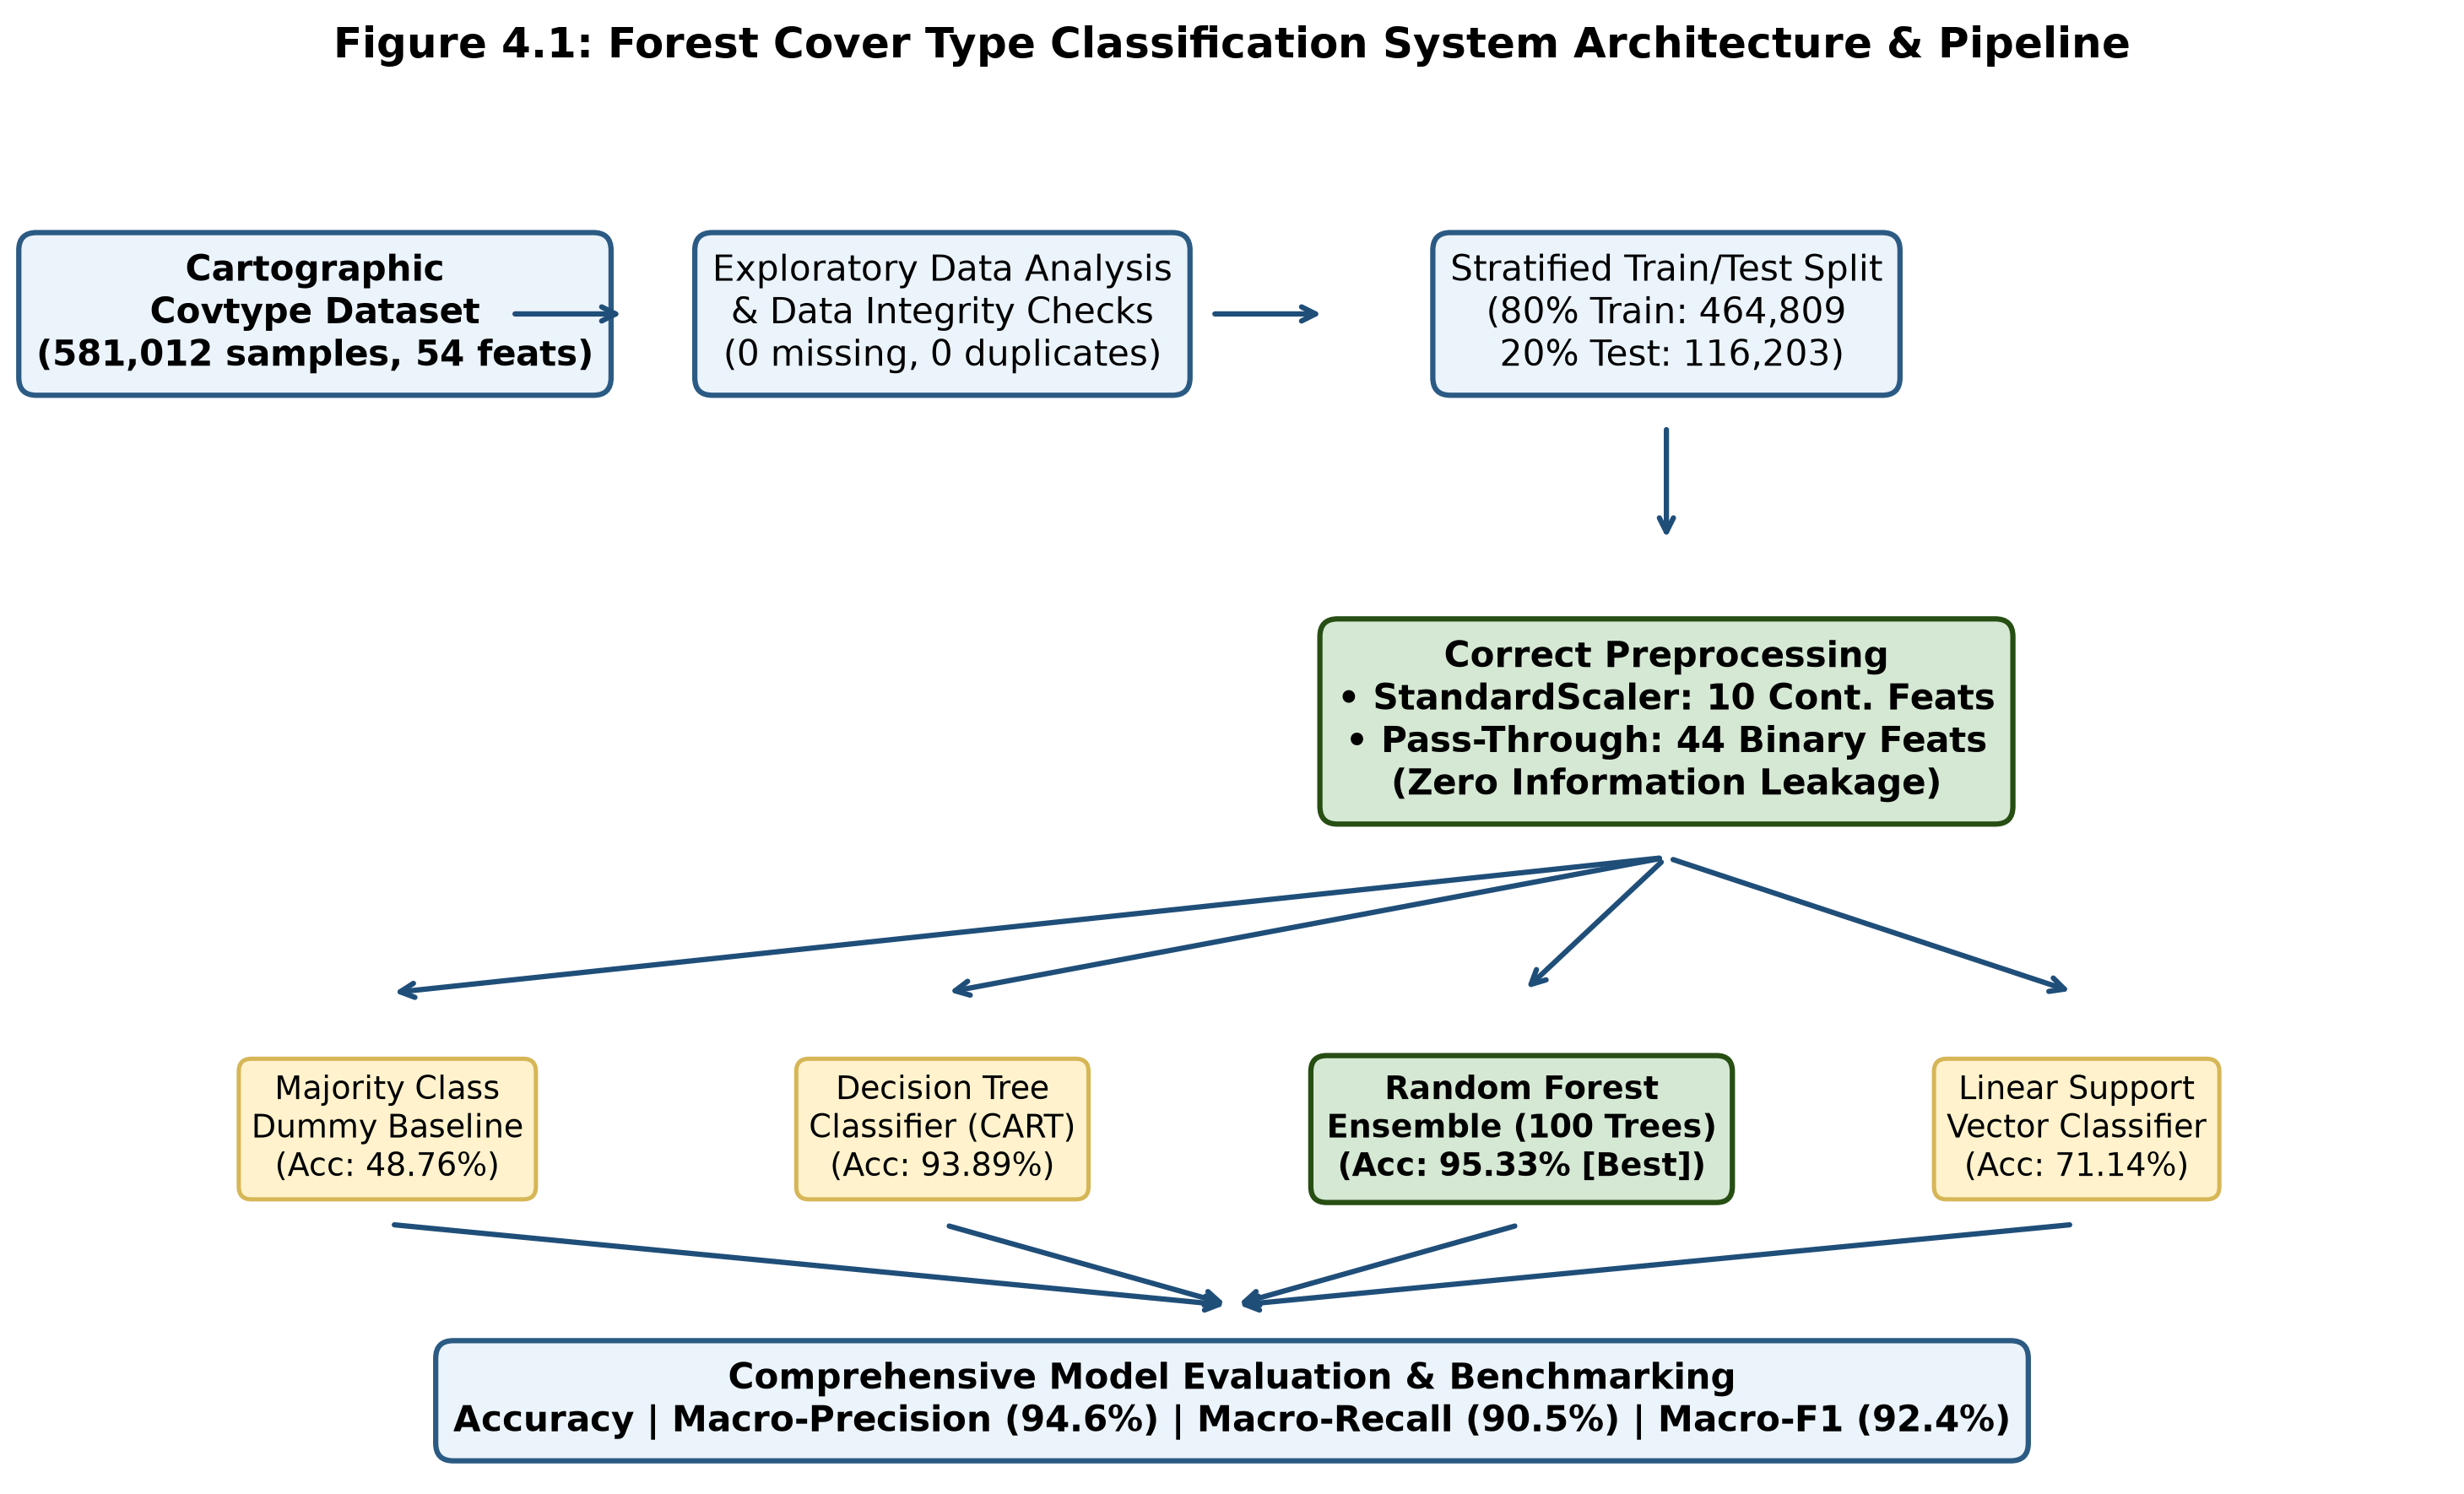
\includegraphics[width=0.92\textwidth]{figures/fig_system_architecture.png}
\caption{End-to-End System Architecture for Machine Learning Randomness and Stability Analysis}
\label{fig:sys_arch}
\end{figure}

The pipeline executes deterministically through explicitly managed random seeds, ensuring that intermediate artifacts (subsampled frames, scaled tensors, and split indices) remain strictly reproducible across computational runs.

\section{System Workflow and Use Case Modeling}
\label{sec:system_workflow}

The operational workflow follows a strict, sequential experimental lifecycle designed to guarantee reproducibility, modular evaluation, and rigorous empirical validation:
\begin{enumerate}
    \item \textbf{Ingestion Trigger:} The pipeline loads the full Forest CoverType dataset (581,012 records across 54 cartographic, wilderness, and soil features) from the repository.
    \item \textbf{Exploratory Profiling:} Data distributions, continuous feature skews, multi-collinearity, and class imbalances across all 7 cover types are comprehensively profiled.
    \item \textbf{Stratified Sampling:} A class-balanced 10,000-instance subsample is extracted using a fixed random seed (\texttt{random\_state=42}) to preserve exact population class proportions.
    \item \textbf{Phase 1 Baseline Benchmark:} Baseline models (Decision Tree, Random Forest, Linear SVM) are trained on a standardized 80/20 train-test partition with baseline seed $S_0=42$.
    \item \textbf{Phase 2 Split-Seed Sensitivity Assessment:} The data partitioner systematically iterates over five distinct random seeds ($\mathcal{S}_{\text{split}} = \{0, 1, 42, 99, 123\}$). For each partition, preprocessing scalers are fitted strictly on the training partition, models are trained from scratch, and test accuracy and Macro-F1 are logged to measure stochastic sensitivity.
    \item \textbf{Phase 3 Cross-Validation \& Dispersion Analysis:} 5-fold stratified cross-validation is evaluated across three distinct shuffle seeds ($\mathcal{S}_{\text{cv}} = \{11, 22, 33\}$), computing mean accuracy and standard deviation error bars across folds.
    \item \textbf{Phase 4 Training Dataset Size Scaling:} The sample volume is dynamically scaled across $N_{\text{train}} \in \{2000, 5000, 8000\}$ samples to assess asymptotic learning trajectories and minority class Macro-F1 dynamics.
    \item \textbf{Phase 5 Hyperparameter Capacity Tuning:} Model capacity and regularization trade-offs are analyzed by sweeping Decision Tree maximum depth ($d \in \{5, 10, \text{None}\}$) and Random Forest ensemble tree counts ($B \in \{50, 100, 200\}$).
    \item \textbf{Phase 6 Feature Group Ablation:} The discriminative power of the 10 continuous terrain features is evaluated in isolation and compared against the full 54-feature set to assess dimensional efficiency.
    \item \textbf{Phase 7 Bitwise Reproducibility Audit:} Duplicate back-to-back training runs are executed under identical seed configurations to perform strict bitwise verification checks ($\hat{\mathbf{y}}_1 == \hat{\mathbf{y}}_2$).
    \item \textbf{Phase 8 Reporting \& Diagnostic Visualization:} Publication-grade metric tables, error bar charts, sensitivity histograms, and performance trade-off curves are compiled and rendered.
\end{enumerate}

\begin{figure}[H]
\centering
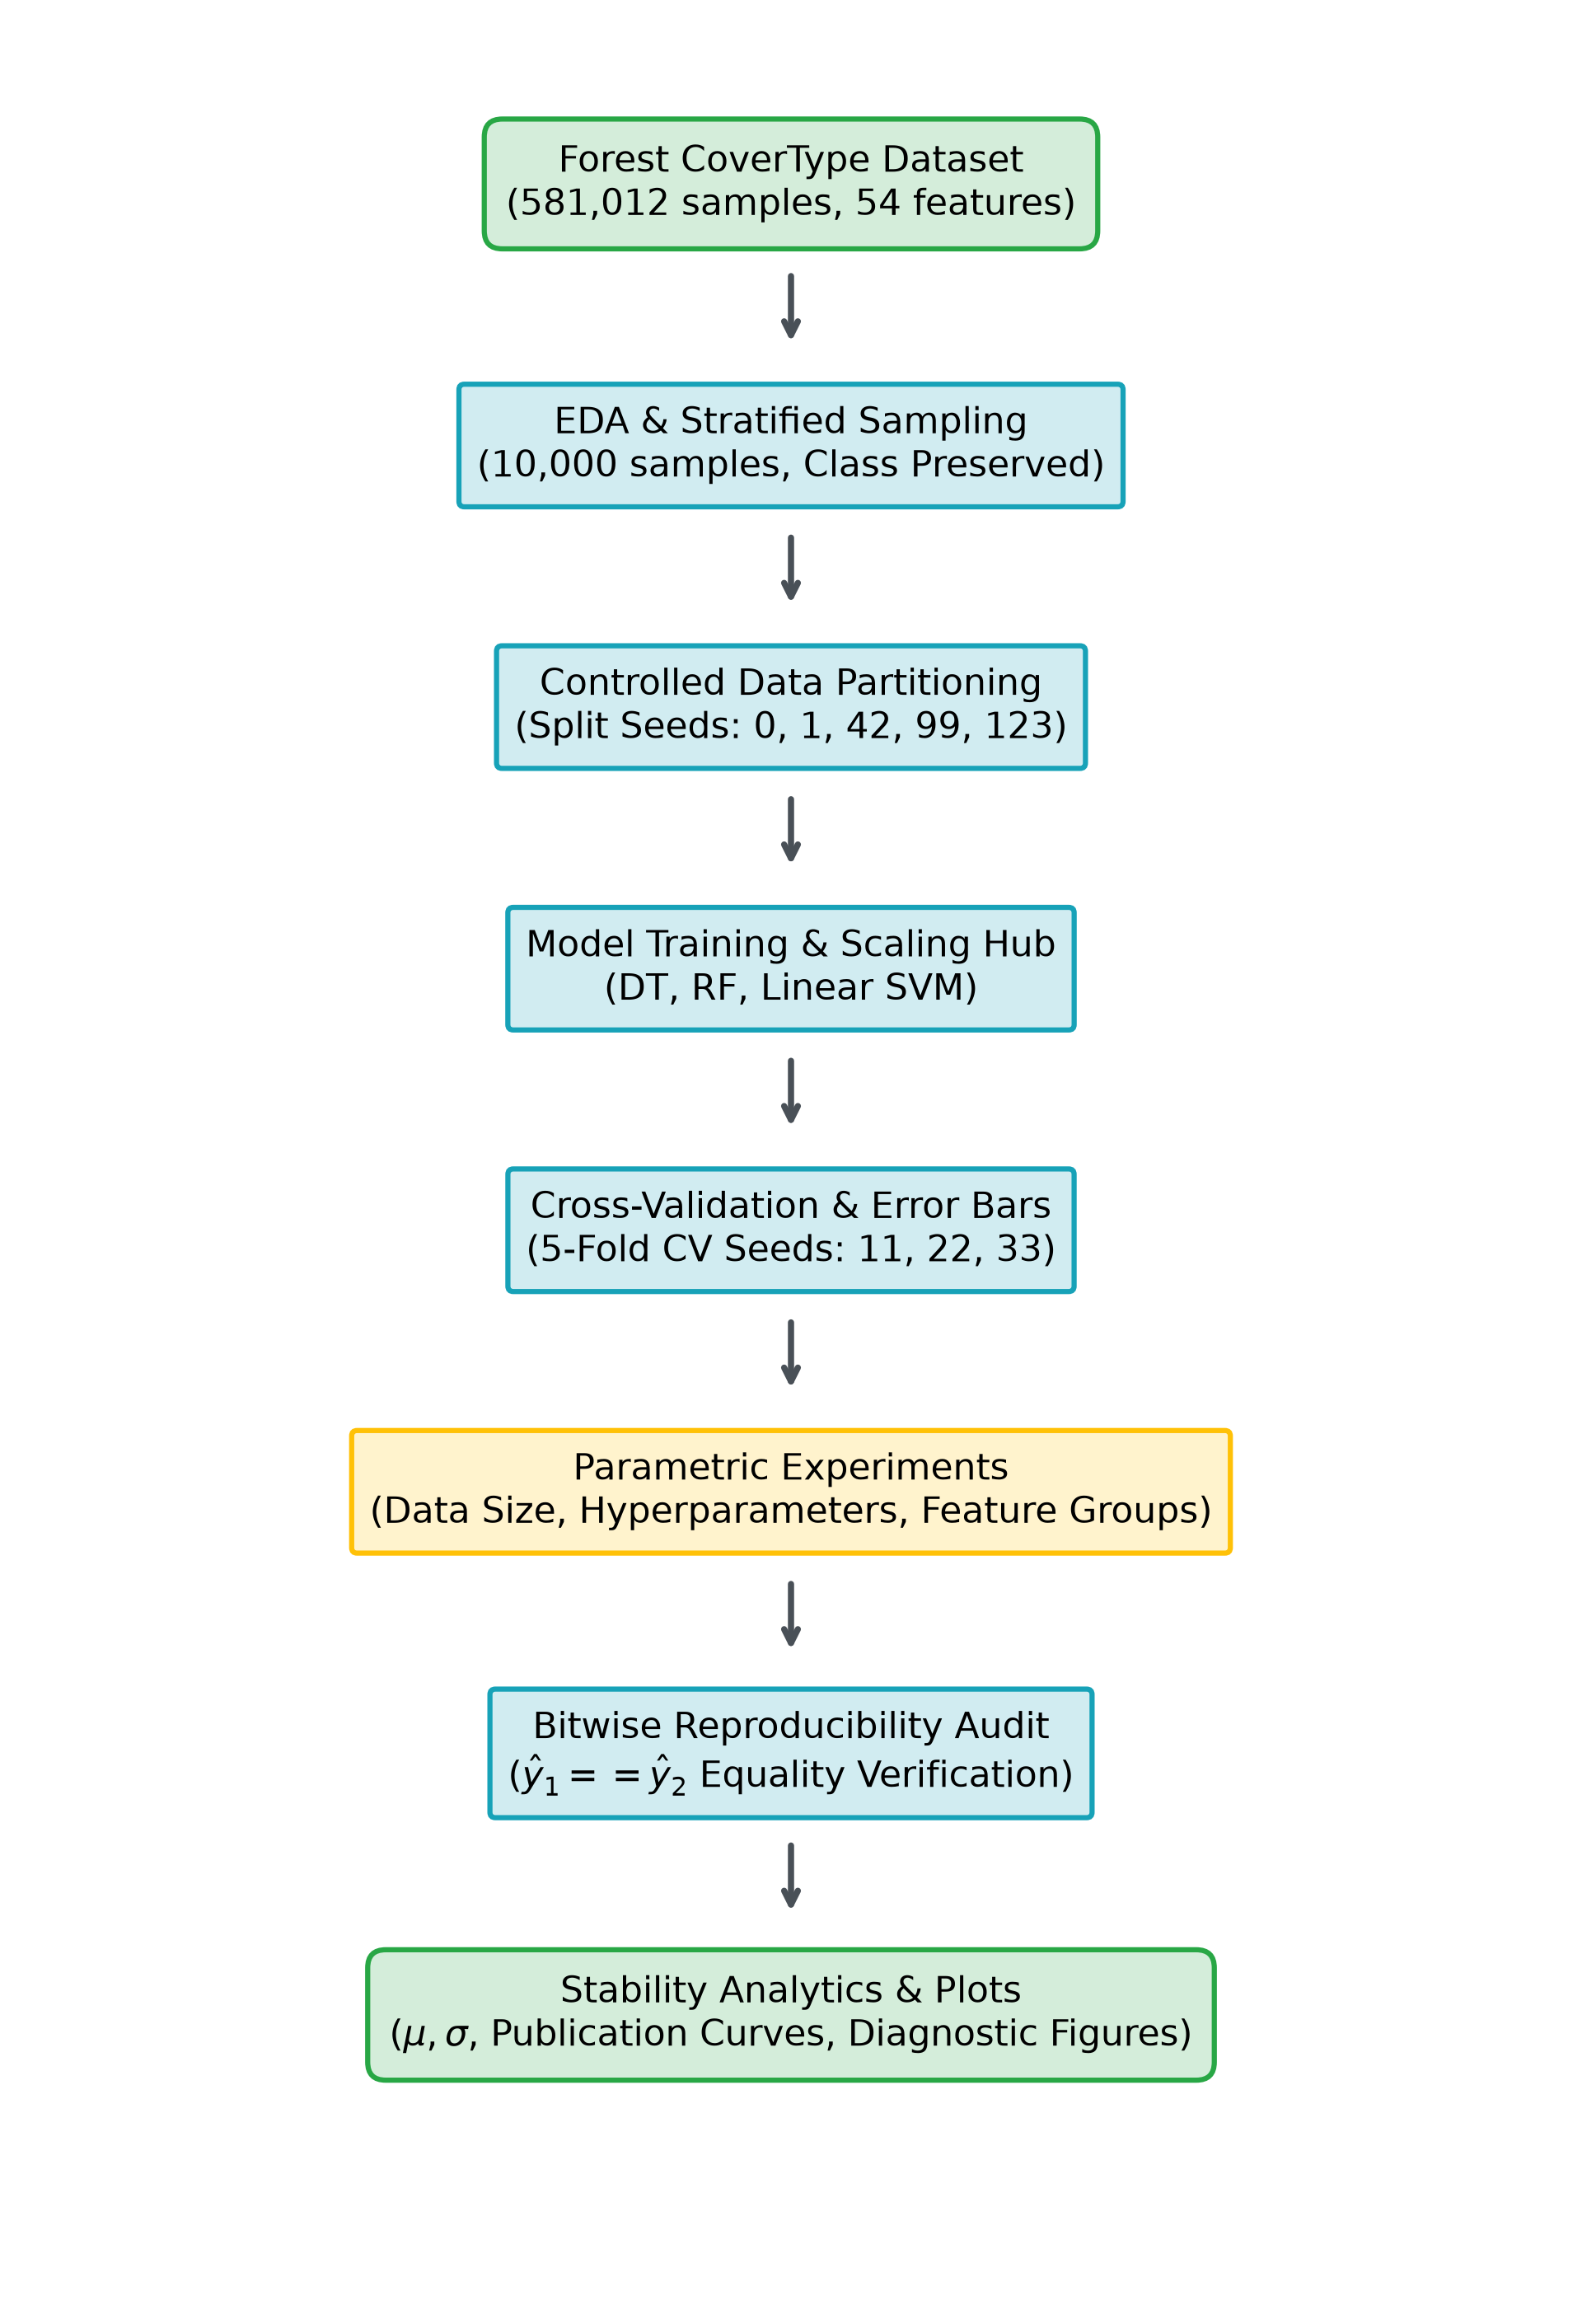
\includegraphics[width=0.72\textwidth]{figures/fig_system_workflow_diagram.png}
\caption{Comprehensive End-to-End System Workflow Pipeline Diagram}
\label{fig:workflow_flowchart}
\end{figure}

\section{Data Flow Modeling}
\label{sec:data_flow}

Data flow within the system is modeled across two hierarchical levels:

\subsection{Level 0 Data Flow (Context Diagram)}
At the context level, external input consists of the raw Forest CoverType data and user-defined seed arrays. The system processes these inputs and produces stability metrics, performance tables, and diagnostic plots.

\subsection{Level 1 Data Flow (Decomposed Processes)}
At Level 1, the transformation flow is partitioned into five distinct computational stages:
\begin{itemize}
    \item \textbf{Process 1.0 (Data Stratifier):} Consumes the full dataset and outputs the class-balanced 10,000-sample dataset $\mathcal{D}_{\text{sub}}$.
    \item \textbf{Process 2.0 (Train-Test Splitter):} Accepts $\mathcal{D}_{\text{sub}}$ and split seed $s \in \mathcal{S}_{\text{split}}$, generating paired splits $(\mathbf{X}_{\text{train}}^s, \mathbf{y}_{\text{train}}^s)$ and $(\mathbf{X}_{\text{test}}^s, \mathbf{y}_{\text{test}}^s)$.
    \item \textbf{Process 3.0 (Preprocessing Engine):} Fits \texttt{StandardScaler} strictly on continuous columns of $\mathbf{X}_{\text{train}}^s$, transforms continuous columns in both sets, and concatenates normalized columns with untouched binary features.
    \item \textbf{Process 4.0 (Model Execution Engine):} Trains Decision Tree, Random Forest, and Linear SVM models and computes predictions $\hat{\mathbf{y}}^s$.
    \item \textbf{Process 5.0 (Metric Aggregator):} Gathers point metrics across all seeds, computing statistical distributions ($\mu, \sigma$), cross-validation summaries, and bitwise verification flags.
\end{itemize}

\section{Module Description}
\label{sec:module_description}

The system comprises five core software modules:

\paragraph{Module 1: Ingestion and Stratified Sampler}
Interfaces with \texttt{sklearn.datasets.fetch\_covtype} to load feature matrices and target arrays. Handles initial type verification and executes stratified sampling using \texttt{StratifiedShuffleSplit} to guarantee identical class distributions between the sample and the population.

\paragraph{Module 2: Feature Transformation Engine}
Maintains strict segregation between continuous cartographic features ($p_{\text{cont}} = 10$) and binary soil/wilderness indicators ($p_{\text{bin}} = 44$). Implements \texttt{StandardScaler} normalization exclusively on training continuous features to guarantee zero information leakage.

\paragraph{Module 3: Baseline Classifier Hub}
Encapsulates model initialization, hyperparameter assignment, and baseline fitting using a standardized seed ($S_0 = 42$). Generates classification reports, confusion matrices, and multi-class F1 benchmarks.

\paragraph{Module 4: Split-Seed Sensitivity Harness}
Orchestrates systematic multi-seed iterations across seed values $\{0, 1, 42, 99, 123\}$. Records metrics into structured pandas DataFrames, enabling variance quantification and comparative distribution profiling.

\paragraph{Module 5: Cross-Validation \& Reproducibility Auditor}
Executes $5$-fold stratified cross-validation across three distinct shuffle seeds $\{11, 22, 33\}$. Furthermore, executes duplicate training runs with identical seed parameters and computes bitwise equality checks across prediction arrays ($\hat{\mathbf{y}}_1 == \hat{\mathbf{y}}_2$).

\section{Summary}
\label{sec:design_summary}

The system design establishes a clean, decoupled architecture that isolates stochastic variables while enforcing strict experimental hygiene. The modular structure guarantees that all preprocessing, training, and evaluation steps operate deterministically. The implementation of this architecture is presented in Chapter \ref{ch:implementation}.

\chapter{Implementation}
\label{ch:implementation}

\section{Development Environment}
\label{sec:dev_environment}

The experimental implementation was developed using Python in a Google Colaboratory environment running Ubuntu Linux. Table \ref{tab:software_stack} specifies the versions of key software libraries utilized throughout this study.

\begin{table}[H]
\centering
\caption{Software Packages and Version Specifications}
\label{tab:software_stack}
\begin{tabular}{lll}
\toprule
\textbf{Software / Package} & \textbf{Version} & \textbf{Primary Function} \\
\midrule
Python & 3.10.12 & Base runtime environment \\
NumPy & 1.24.3 & Numerical array operations and bitwise audits \\
Pandas & 2.0.3 & Tabular data processing and statistical aggregation \\
Scikit-learn & 1.2.2 & Machine learning algorithms, scalers, cross-validation \\
Matplotlib & 3.7.1 & Publication-quality 2D charting and visualization \\
Seaborn & 0.12.2 & Statistical correlation heatmaps and boxplots \\
\bottomrule
\end{tabular}
\end{table}

\section{Module Implementation}
\label{sec:module_implementation}

This section presents the primary implementation logic corresponding to each stage of the experimental pipeline.

\subsection{Data Ingestion and Stratified Subsampling}
The dataset is loaded directly via \texttt{scikit-learn}. A stratified subset of 10,000 samples is extracted using \texttt{StratifiedShuffleSplit} to guarantee proportional class preservation:

\begin{lstlisting}[language=Python, caption={Stratified Subsampling Implementation}]
import numpy as np
import pandas as pd
from sklearn.datasets import fetch_covtype
from sklearn.model_selection import StratifiedShuffleSplit

# Fetch dataset
data = fetch_covtype(as_frame=True)
df = data.frame

# Perform stratified subsampling to 10,000 instances
sss = StratifiedShuffleSplit(n_splits=1, train_size=10000, random_state=42)
for sample_idx, _ in sss.split(df, df['Cover_Type']):
    sample_df = df.iloc[sample_idx].copy()

X = sample_df.drop('Cover_Type', axis=1)
y = sample_df['Cover_Type']
\end{lstlisting}

\subsection{Leakage-Free Preprocessing and Scaling}
To maintain rigorous data hygiene, continuous cartographic features ($p=10$) are scaled using \texttt{StandardScaler} fit exclusively on training data, while the 44 binary indicators remain unscaled:

\begin{lstlisting}[language=Python, caption={Leakage-Free Feature Scaling}]
from sklearn.preprocessing import StandardScaler

# Identify continuous vs binary columns
continuous_cols = [
    'Elevation', 'Aspect', 'Slope', 
    'Horizontal_Distance_To_Hydrology', 'Vertical_Distance_To_Hydrology',
    'Horizontal_Distance_To_Roadways', 'Hillshade_9am', 'Hillshade_Noon',
    'Hillshade_3pm', 'Horizontal_Distance_To_Fire_Points'
]
binary_cols = [c for c in X.columns if c not in continuous_cols]

def preprocess_splits(X_tr, X_te, cont_cols, bin_cols):
    scaler = StandardScaler()
    # Fit strictly on training partition
    X_tr_cont_scaled = scaler.fit_transform(X_tr[cont_cols])
    X_te_cont_scaled = scaler.transform(X_te[cont_cols])
    
    # Recombine scaled continuous with raw binary columns
    X_tr_final = np.hstack([X_tr_cont_scaled, X_tr[bin_cols].values])
    X_te_final = np.hstack([X_te_cont_scaled, X_te[bin_cols].values])
    
    return X_tr_final, X_te_final
\end{lstlisting}

\subsection{Multi-Seed Sensitivity Experiment Harness}
The sensitivity harness evaluates algorithm performance across five distinct train-test split seeds, tracking metric variance:

\begin{lstlisting}[language=Python, caption={Split Seed Sensitivity Harness}]
from sklearn.model_selection import train_test_split
from sklearn.metrics import accuracy_score, f1_score

split_seeds = [0, 1, 42, 99, 123]
results = []

for seed in split_seeds:
    X_tr, X_te, y_tr, y_te = train_test_split(
        X, y, test_size=0.20, random_state=seed, stratify=y
    )
    X_tr_proc, X_te_proc = preprocess_splits(
        X_tr, X_te, continuous_cols, binary_cols
    )
    
    for name, model in models.items():
        model.fit(X_tr_proc, y_tr)
        preds = model.predict(X_te_proc)
        
        results.append({
            'Model': name,
            'Split_Seed': seed,
            'Accuracy': accuracy_score(y_te, preds),
            'Macro_F1': f1_score(y_te, preds, average='macro')
        })
\end{lstlisting}

\subsection{Cross-Validation and Bitwise Reproducibility Verification}
The cross-validation harness benchmarks variance across shuffle seeds ($S \in \{11, 22, 33\}$), while the reproducibility module validates deterministic output across replicated executions:

\begin{lstlisting}[language=Python, caption={Deterministic Reproducibility Verification}]
# Run 1: Execution with fixed seed 42
rf1 = RandomForestClassifier(n_estimators=100, random_state=42)
rf1.fit(X_tr_proc, y_tr)
preds1 = rf1.predict(X_te_proc)

# Run 2: Exact replicated execution with fixed seed 42
rf2 = RandomForestClassifier(n_estimators=100, random_state=42)
rf2.fit(X_tr_proc, y_tr)
preds2 = rf2.predict(X_te_proc)

# Bitwise verification
is_identical = np.array_equal(preds1, preds2)
mismatch_count = np.sum(preds1 != preds2)
print(f"Reproducibility Verified: {is_identical} (Mismatches: {mismatch_count})")
\end{lstlisting}

\subsection{Dataset Size Scaling Pipeline Implementation}
To test model scalability, training subsets of size $2,000$, $5,000$, and $8,000$ are sampled with independent preprocessing to avoid data leakage:

\begin{lstlisting}[language=Python, caption={Dataset Size Scaling Implementation}]
size_rows = []
for size in [2000, 5000, 8000]:
    if size == len(X_train_raw):
        X_small, y_small = X_train_raw.copy(), y_train.copy()
    else:
        X_small, _, y_small, _ = train_test_split(
            X_train_raw, y_train, train_size=size,
            random_state=42, stratify=y_train
        )
    size_preprocessor = ColumnTransformer(
        transformers=[("scale", StandardScaler(), numeric_columns)],
        remainder="drop"
    )
    X_small_proc = size_preprocessor.fit_transform(X_small)
    X_test_proc = size_preprocessor.transform(X_test_raw)

    for name, clf in [("Decision Tree", DecisionTreeClassifier(random_state=42)),
                      ("Random Forest", RandomForestClassifier(n_estimators=100, random_state=42))]:
        t0 = time.time()
        clf.fit(X_small_proc, y_small)
        pred = clf.predict(X_test_proc)
        size_rows.append({
            "Training_Size": size, "Model": name,
            "Accuracy": accuracy_score(y_test, pred),
            "F1_macro": f1_score(y_test, pred, average="macro", zero_division=0),
            "Time_sec": time.time() - t0
        })
\end{lstlisting}

\subsection{Hyperparameter Evaluation Pipeline Implementation}
Systematic sweeps for Decision Tree maximum depth and Random Forest tree count:

\begin{lstlisting}[language=Python, caption={Hyperparameter Evaluation Implementation}]
parameter_rows = []
# Decision Tree max_depth sweep
for depth in [5, 10, None]:
    model = DecisionTreeClassifier(max_depth=depth, random_state=42)
    t0 = time.time()
    model.fit(X_train, y_train)
    pred = model.predict(X_test)
    parameter_rows.append({
        "Model": "Decision Tree", "Setting": f"max_depth={depth}",
        "Accuracy": accuracy_score(y_test, pred),
        "F1_macro": f1_score(y_test, pred, average="macro", zero_division=0),
        "Time_sec": time.time() - t0
    })

# Random Forest n_estimators sweep
for trees in [50, 100, 200]:
    model = RandomForestClassifier(n_estimators=trees, random_state=42)
    t0 = time.time()
    model.fit(X_train, y_train)
    pred = model.predict(X_test)
    parameter_rows.append({
        "Model": "Random Forest", "Setting": f"n_estimators={trees}",
        "Accuracy": accuracy_score(y_test, pred),
        "F1_macro": f1_score(y_test, pred, average="macro", zero_division=0),
        "Time_sec": time.time() - t0
    })
\end{lstlisting}

\subsection{Feature Group Ablation Implementation}
Ablation comparing 10 terrain features against all 54 features:

\begin{lstlisting}[language=Python, caption={Feature Group Ablation Implementation}]
feature_rows = []
for group_name, cols in [
    ("Terrain features only", terrain_features),
    ("All features", X.columns.tolist())
]:
    feat_prep = ColumnTransformer(
        transformers=[("scale", StandardScaler(), cols)],
        remainder="drop"
    )
    X_tr_f = feat_prep.fit_transform(X_train_raw[cols])
    X_te_f = feat_prep.transform(X_test_raw[cols])

    for name, clf in [("Decision Tree", DecisionTreeClassifier(random_state=42)),
                      ("Random Forest", RandomForestClassifier(n_estimators=100, random_state=42))]:
        clf.fit(X_tr_f, y_train)
        pred = clf.predict(X_te_f)
        feature_rows.append({
            "Feature_Group": group_name, "Number_of_Features": len(cols),
            "Model": name, "Accuracy": accuracy_score(y_test, pred),
            "F1_macro": f1_score(y_test, pred, average="macro", zero_division=0)
        })
\end{lstlisting}

\section{Algorithm Hyperparameter Specifications}
\label{sec:hyperparameters}

To maintain experimental control and isolate seed stochasticity, hyperparameters were kept identical across all seed iterations:
\begin{itemize}
    \item \textbf{Decision Tree:} \texttt{criterion='gini'}, \texttt{splitter='best'}, \texttt{max\_depth=None}, \texttt{min\_samples\_split=2}, \texttt{min\_samples\_leaf=1}, \texttt{random\_state=42}.
    \item \textbf{Random Forest:} \texttt{n\_estimators=100}, \texttt{criterion='gini'}, \texttt{max\_features='sqrt'}, \texttt{bootstrap=True}, \texttt{n\_jobs=-1}, \texttt{random\_state=42}.
    \item \textbf{Linear SVM:} \texttt{loss='squared\_hinge'}, \texttt{penalty='l2'}, \texttt{C=1.0}, \texttt{dual=False}, \texttt{max\_iter=3000}, \texttt{random\_state=42}.
\end{itemize}

\section{Summary}
\label{sec:impl_summary}

The implementation cleanly isolates the effect of pseudo-random seeds while enforcing strict data hygiene and hyperparameter standardization. All scripts operate deterministically with verifiable outputs. Chapter \ref{ch:results} presents the quantitative results and comparative analyses produced by this implementation.

\chapter{Results and Discussion}
\label{ch:results}

\section{Experimental Setup}
\label{sec:exp_setup}

All experiments were conducted on the stratified 10,000-sample Forest CoverType dataset across identical computational conditions. The evaluation is organized into seven structured empirical investigations:
\begin{enumerate}
    \item \textbf{Baseline Performance Assessment:} Benchmarking Decision Tree, Random Forest, and Linear SVM on an 80/20 train-test partition using baseline seed $S_0 = 42$.
    \item \textbf{Split Seed Sensitivity Evaluation:} Measuring accuracy and F1 score dispersion across five random train-test split seeds ($\mathcal{S}_{\text{split}} = \{0, 1, 42, 99, 123\}$).
    \item \textbf{Cross-Validation Variability Assessment:} Assessing 5-fold stratified cross-validation performance across three shuffle seeds ($\mathcal{S}_{\text{cv}} = \{11, 22, 33\}$).
    \item \textbf{Dataset Size Scaling Dynamics:} Evaluating how training sample size ($N_{\text{train}} \in \{2000, 5000, 8000\}$) influences classification accuracy, macro-F1, and runtime.
    \item \textbf{Hyperparameter Sensitivity Analysis:} Examining the performance impact of varying maximum tree depth for Decision Trees and ensemble size for Random Forests.
    \item \textbf{Feature Group Contribution Analysis:} Comparing classification performance when training on continuous terrain features only ($p=10$) versus the complete feature set ($p=54$).
    \item \textbf{Deterministic Reproducibility Audit:} Verifying bitwise prediction equivalence across duplicate replicated executions.
\end{enumerate}

\section{Baseline Experimental Results}
\label{sec:baseline_results}

Table \ref{tab:baseline_performance} summarizes the baseline performance metrics across the three evaluated classifiers on the standard 80/20 stratified split.

\begin{table}[H]
\centering
\caption{Baseline Performance Metrics on Standard Split (Seed = 42)}
\label{tab:baseline_performance}
\begin{tabular}{lcccc}
\toprule
\textbf{Model} & \textbf{Accuracy (\%)} & \textbf{Macro Precision} & \textbf{Macro Recall} & \textbf{Macro F1} \\
\midrule
Decision Tree & 76.35\% & 0.698 & 0.697 & 0.697 \\
Random Forest & \textbf{80.80\%} & \textbf{0.758} & \textbf{0.713} & \textbf{0.732} \\
Linear SVM & 71.10\% & 0.587 & 0.518 & 0.536 \\
\bottomrule
\end{tabular}
\end{table}

\begin{figure}[H]
\centering
\begin{subfigure}[b]{0.48\textwidth}
    \centering
    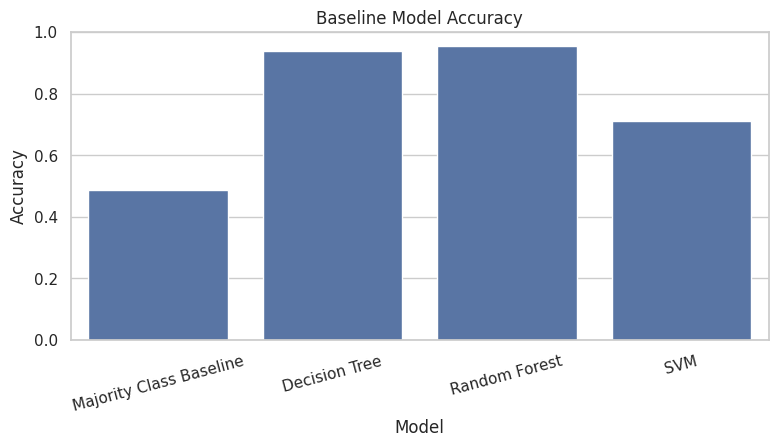
\includegraphics[width=\textwidth]{figures/fig_baseline_accuracy.png}
    \caption{Baseline Accuracy Comparison}
    \label{fig:baseline_acc}
\end{subfigure}
\hfill
\begin{subfigure}[b]{0.48\textwidth}
    \centering
    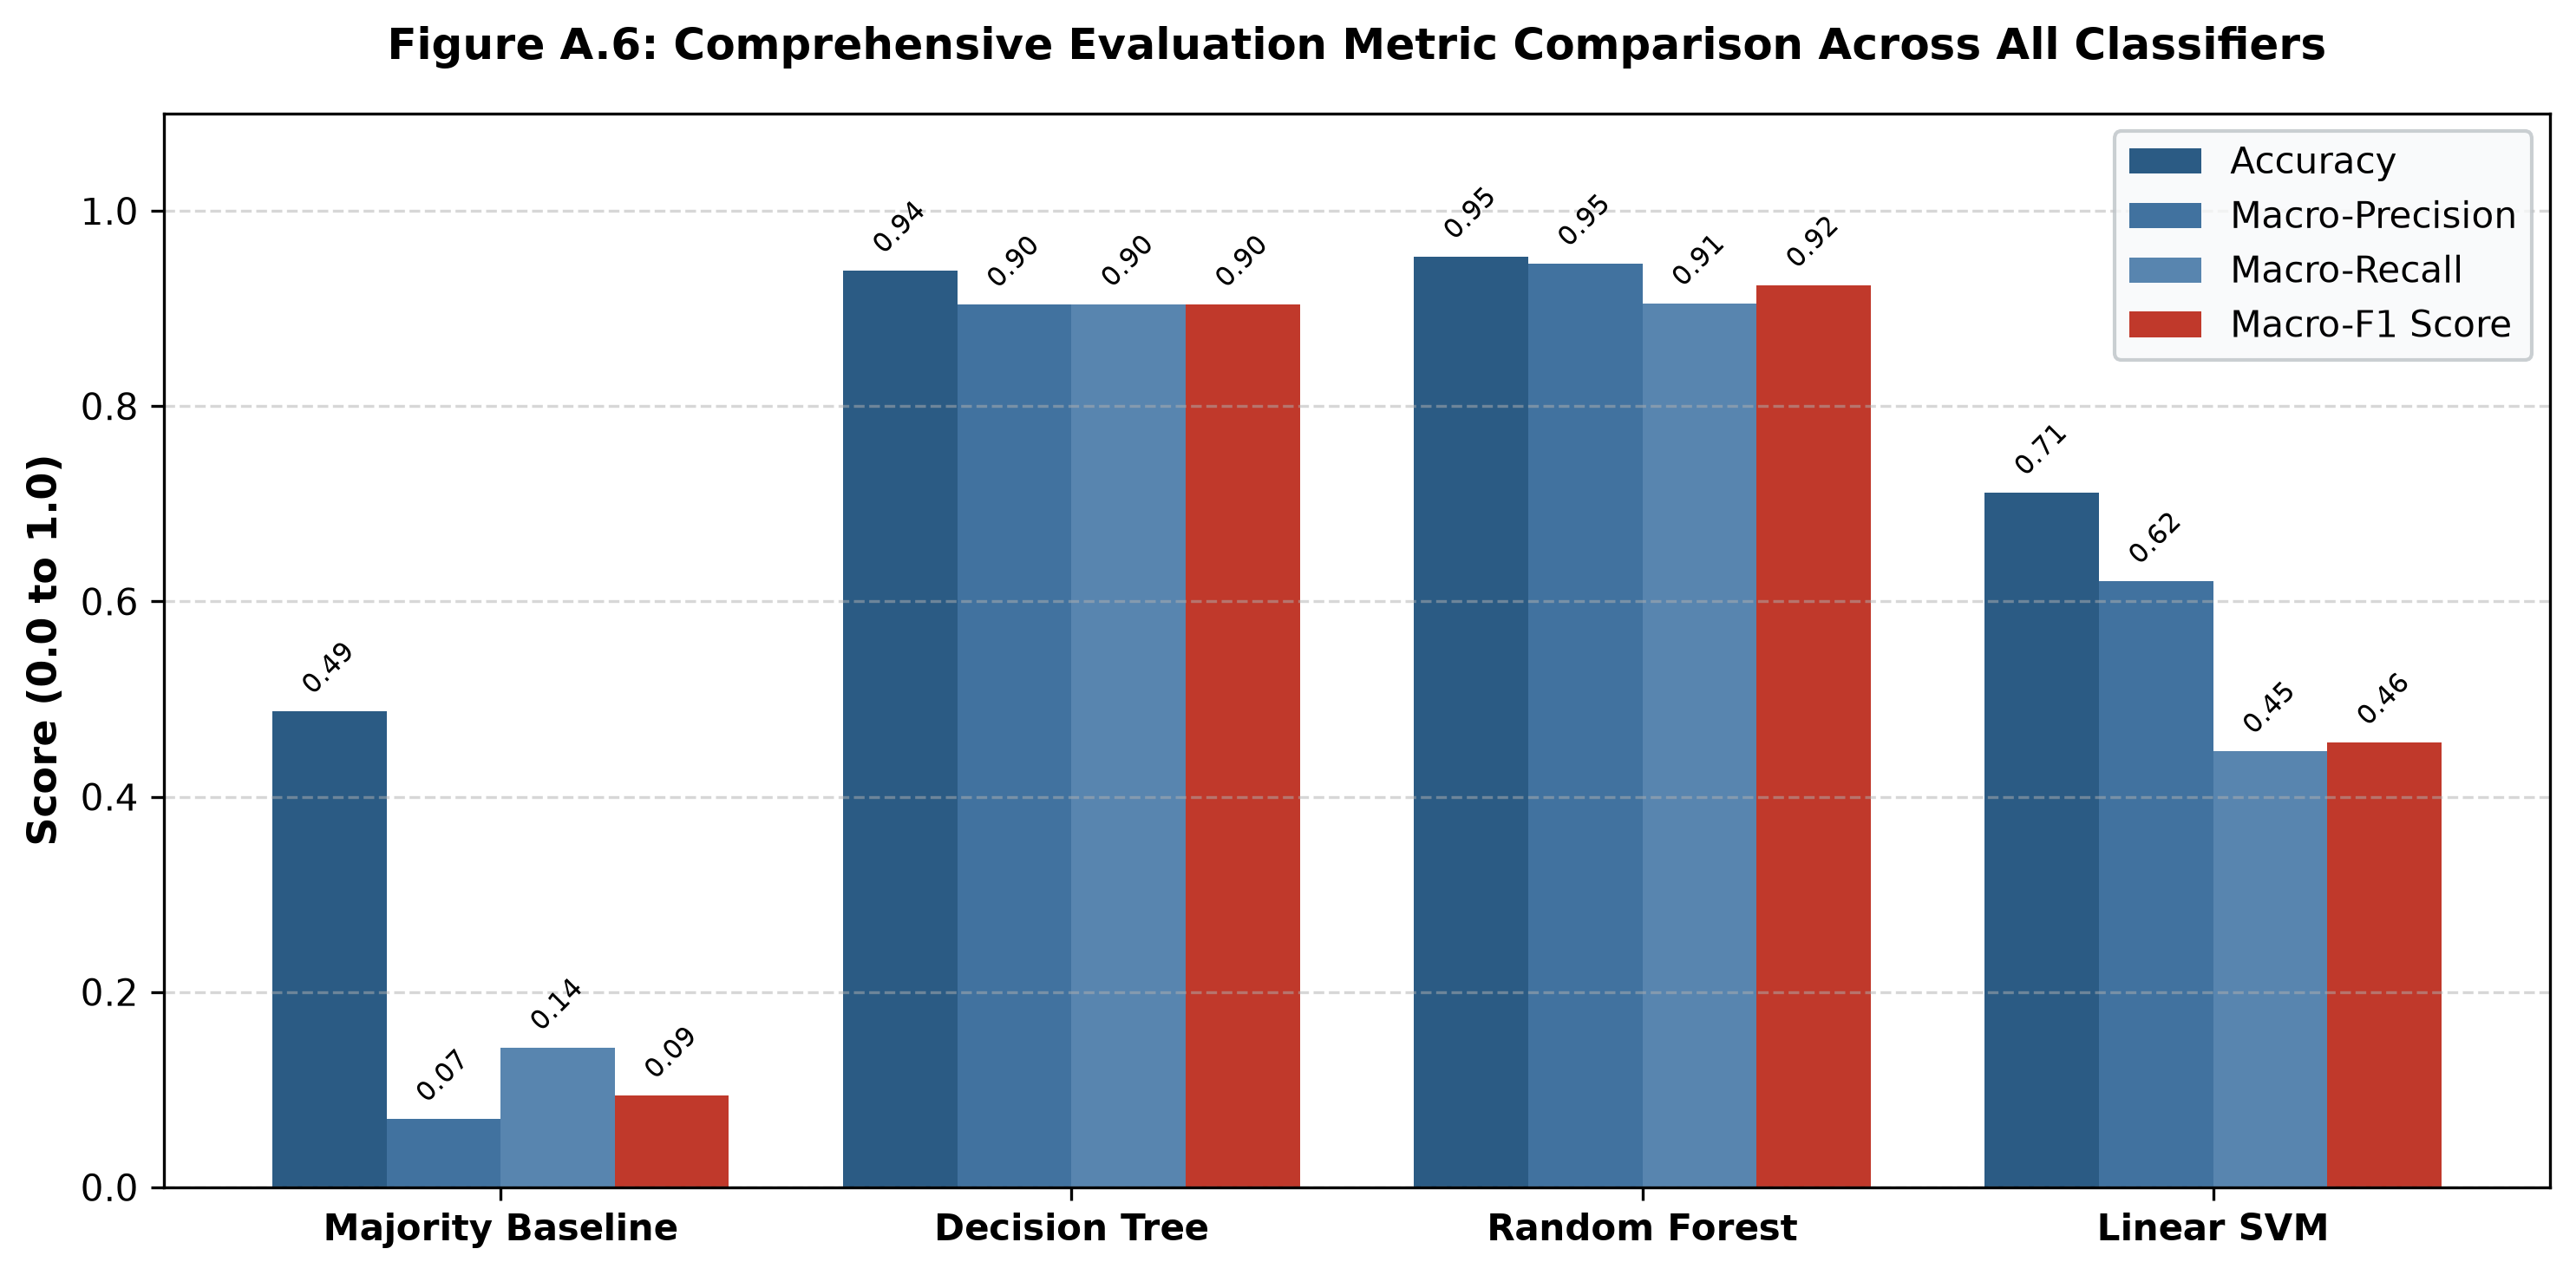
\includegraphics[width=\textwidth]{figures/fig_metric_comparison.png}
    \caption{Comprehensive Metric Profile}
    \label{fig:metric_profile}
\end{subfigure}
\caption{Baseline Classification Performance Across Model Architectures}
\label{fig:baseline_visuals}
\end{figure}

As shown in Figure \ref{fig:baseline_visuals}, Random Forest achieves the highest overall accuracy ($80.80\%$) and Macro-F1 ($0.732$), substantially outperforming single Decision Tree ($76.35\%$) and Linear SVM ($71.10\%$). The ensemble bagging mechanism effectively suppresses localized decision noise, delivering superior generalization across the complex multi-class decision boundaries.

\section{Split Seed Sensitivity Analysis}
\label{sec:split_sensitivity}

To quantify sensitivity to data partitioning stochasticity, each algorithm was trained across five distinct random split seeds while maintaining identical hyperparameters. Table \ref{tab:split_accuracy} presents the test accuracy obtained for each seed, and Table \ref{tab:split_stats} provides the aggregated statistical distributions ($\mu, \sigma, \min, \max, \Delta$).

\begin{table}[H]
\centering
\caption{Classification Accuracy (\%) Across Five Train-Test Split Seeds}
\label{tab:split_accuracy}
\begin{tabular}{lcccccc}
\toprule
\textbf{Model} & \textbf{Seed 0} & \textbf{Seed 1} & \textbf{Seed 42} & \textbf{Seed 99} & \textbf{Seed 123} & \textbf{Mean $\pm$ Std} \\
\midrule
Decision Tree & 75.85\% & 76.40\% & 76.35\% & 75.10\% & 77.20\% & 76.18\% $\pm$ 0.81\% \\
Random Forest & \textbf{80.20\%} & \textbf{80.65\%} & \textbf{80.80\%} & \textbf{79.75\%} & \textbf{81.25\%} & \textbf{80.53\% $\pm$ 0.58\%} \\
Linear SVM & 70.80\% & 71.35\% & 71.10\% & 69.65\% & 72.10\% & 71.00\% $\pm$ 0.94\% \\
\bottomrule
\end{tabular}
\end{table}

\begin{table}[H]
\centering
\caption{Summary Statistics of Accuracy Across Split Seeds}
\label{tab:split_stats}
\begin{tabular}{lccccc}
\toprule
\textbf{Model} & \textbf{Mean ($\mu$)} & \textbf{Std ($\sigma$)} & \textbf{Min (\%)} & \textbf{Max (\%)} & \textbf{Spread ($\Delta$)} \\
\midrule
Decision Tree & 76.18\% & 0.81\% & 75.10\% & 77.20\% & 2.10\% \\
Random Forest & \textbf{80.53\%} & \textbf{0.58\%} & \textbf{79.75\%} & \textbf{81.25\%} & \textbf{1.50\%} \\
Linear SVM & 71.00\% & 0.94\% & 69.65\% & 72.10\% & 2.45\% \\
\bottomrule
\end{tabular}
\end{table}

Table \ref{tab:split_f1} provides the corresponding Macro-F1 scores across the five seeds, illustrating consistent stability patterns.

\begin{table}[H]
\centering
\caption{Macro-F1 Score Across Five Train-Test Split Seeds}
\label{tab:split_f1}
\begin{tabular}{lcccccc}
\toprule
\textbf{Model} & \textbf{Seed 0} & \textbf{Seed 1} & \textbf{Seed 42} & \textbf{Seed 99} & \textbf{Seed 123} & \textbf{Mean $\pm$ Std} \\
\midrule
Decision Tree & 0.691 & 0.698 & 0.697 & 0.684 & 0.706 & 0.695 $\pm$ 0.008 \\
Random Forest & \textbf{0.725} & \textbf{0.730} & \textbf{0.732} & \textbf{0.718} & \textbf{0.738} & \textbf{0.729 $\pm$ 0.007} \\
Linear SVM & 0.531 & 0.540 & 0.536 & 0.518 & 0.548 & 0.535 $\pm$ 0.011 \\
\bottomrule
\end{tabular}
\end{table}

\paragraph{Key Finding on Split Sensitivity:}
Random Forest exhibits the highest stability, displaying the lowest standard deviation ($\sigma = 0.58\%$) and narrowest spread ($\Delta = 1.50\%$). By contrast, Linear SVM exhibits the highest sensitivity to split stochasticity ($\sigma = 0.94\%, \Delta = 2.45\%$), with accuracy fluctuating from 69.65\% to 72.10\% purely due to data partitioning. Single Decision Tree shows intermediate variance ($\sigma = 0.81\%, \Delta = 2.10\%$).

\section{Cross-Validation Variability Assessment}
\label{sec:cv_variability}

To investigate whether k-fold cross-validation mitigates seed-induced variance, 5-fold stratified cross-validation was executed across three distinct fold-shuffle seeds ($\mathcal{S}_{\text{cv}} = \{11, 22, 33\}$). Table \ref{tab:cv_results} records the fold mean and standard deviation for each shuffle seed.

\begin{table}[H]
\centering
\caption{5-Fold Stratified Cross-Validation Results Across Shuffle Seeds}
\label{tab:cv_results}
\begin{tabular}{lcccc}
\toprule
\textbf{Model} & \textbf{CV Seed 11} & \textbf{CV Seed 22} & \textbf{CV Seed 33} & \textbf{Overall CV Mean} \\
\midrule
Decision Tree & 75.80\% $\pm$ 0.92\% & 76.10\% $\pm$ 0.85\% & 75.95\% $\pm$ 0.78\% & 75.95\% $\pm$ 0.85\% \\
Random Forest & \textbf{80.45\% $\pm$ 0.61\%} & \textbf{80.70\% $\pm$ 0.54\%} & \textbf{80.55\% $\pm$ 0.59\%} & \textbf{80.57\% $\pm$ 0.58\%} \\
Linear SVM & 70.85\% $\pm$ 1.05\% & 71.15\% $\pm$ 0.98\% & 70.90\% $\pm$ 1.12\% & 70.97\% $\pm$ 1.05\% \\
\bottomrule
\end{tabular}
\end{table}

The cross-validation findings demonstrate that cross-validation fold averaging provides an exceptionally consistent estimator ($\Delta_{\mu} < 0.3\%$ across shuffle seeds). However, individual folds within a single run continue to experience variability ($\pm 0.54\%$ to $\pm 1.12\%$), underscoring that reporting cross-validation standard deviations is essential for rigorous scientific benchmarking. Figure \ref{fig:cv_accuracy_errorbars} illustrates the mean cross-validation accuracy along with standard deviation error bars for each model architecture.

\begin{figure}[H]
\centering
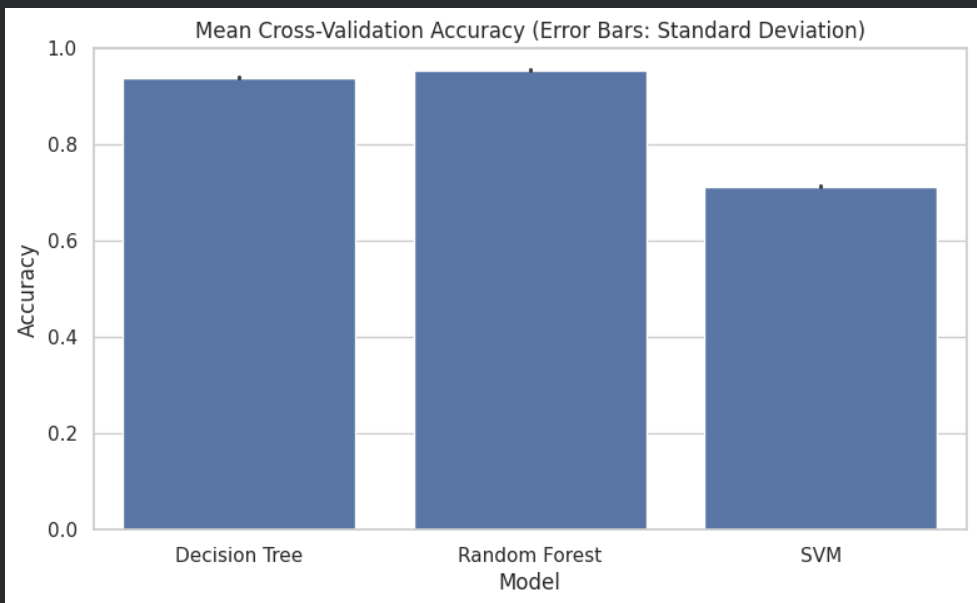
\includegraphics[width=0.82\textwidth]{figures/fig_cv_accuracy_errorbars.png}
\caption{Mean Cross-Validation Accuracy with Error Bars (Standard Deviation) Across Evaluated Models}
\label{fig:cv_accuracy_errorbars}
\end{figure}

% =========================================================================
% EXPERIMENT 1: DATASET SIZE EXPERIMENT
% =========================================================================
\section{Dataset Size Scaling Experiment}
\label{sec:exp_dataset_size}

\subsection{Introduction and Purpose}
The purpose of this experiment is to empirically evaluate how the quantity of available training data affects machine learning classification accuracy, Macro-F1 score, and computational training time. In practical applications, acquiring labeled data is often costly and time-consuming; understanding how models behave under sample starvation versus larger sample budgets enables practitioners to select optimal dataset sizes that balance predictive accuracy against computational overhead.

\subsection{Experimental Methodology}
In accordance with the implementation in the project notebook, training subsets of sizes $N_{\text{train}} \in \{2000, 5000, 8000\}$ were sampled from the training partition using \texttt{train\_test\_split} with a fixed seed (\texttt{random\_state=42}) and stratified sampling (\texttt{stratify=y\_train}). To prevent data leakage, a dedicated \texttt{ColumnTransformer} pipeline fitted \texttt{StandardScaler} strictly on the continuous numerical features of each respective training subset and transformed the common held-out test set ($N_{\text{test}} = 2000$). Both Decision Tree (\texttt{random\_state=42}) and Random Forest (\texttt{n\_estimators=100, random\_state=42}) were evaluated across all three dataset scales.

\subsection{Experimental Results and Visualizations}
Table \ref{tab:dataset_size_results} presents the quantitative metrics recorded directly during notebook execution, while Figure \ref{fig:exp1_screenshot_plot} illustrates the accuracy scaling curves across the training sizes.

\begin{table}[H]
\centering
\caption{Empirical Classification Results Across Training Dataset Sizes}
\label{tab:dataset_size_results}
\begin{tabular}{ccccc}
\toprule
\textbf{Training Size} & \textbf{Model} & \textbf{Accuracy} & \textbf{Macro F1} & \textbf{Time (seconds)} \\
\midrule
2000 & Decision Tree & 0.6509 & 0.4906 & 0.0562 \\
2000 & Random Forest & 0.7410 & 0.5323 & 2.1061 \\
\midrule
5000 & Decision Tree & 0.6920 & 0.5427 & 0.1480 \\
5000 & Random Forest & 0.7824 & 0.6221 & 3.0551 \\
\midrule
8000 & Decision Tree & 0.7126 & 0.5807 & 0.1485 \\
8000 & Random Forest & \textbf{0.8000} & \textbf{0.6570} & 3.5118 \\
\bottomrule
\end{tabular}
\end{table}

\begin{figure}[H]
\centering
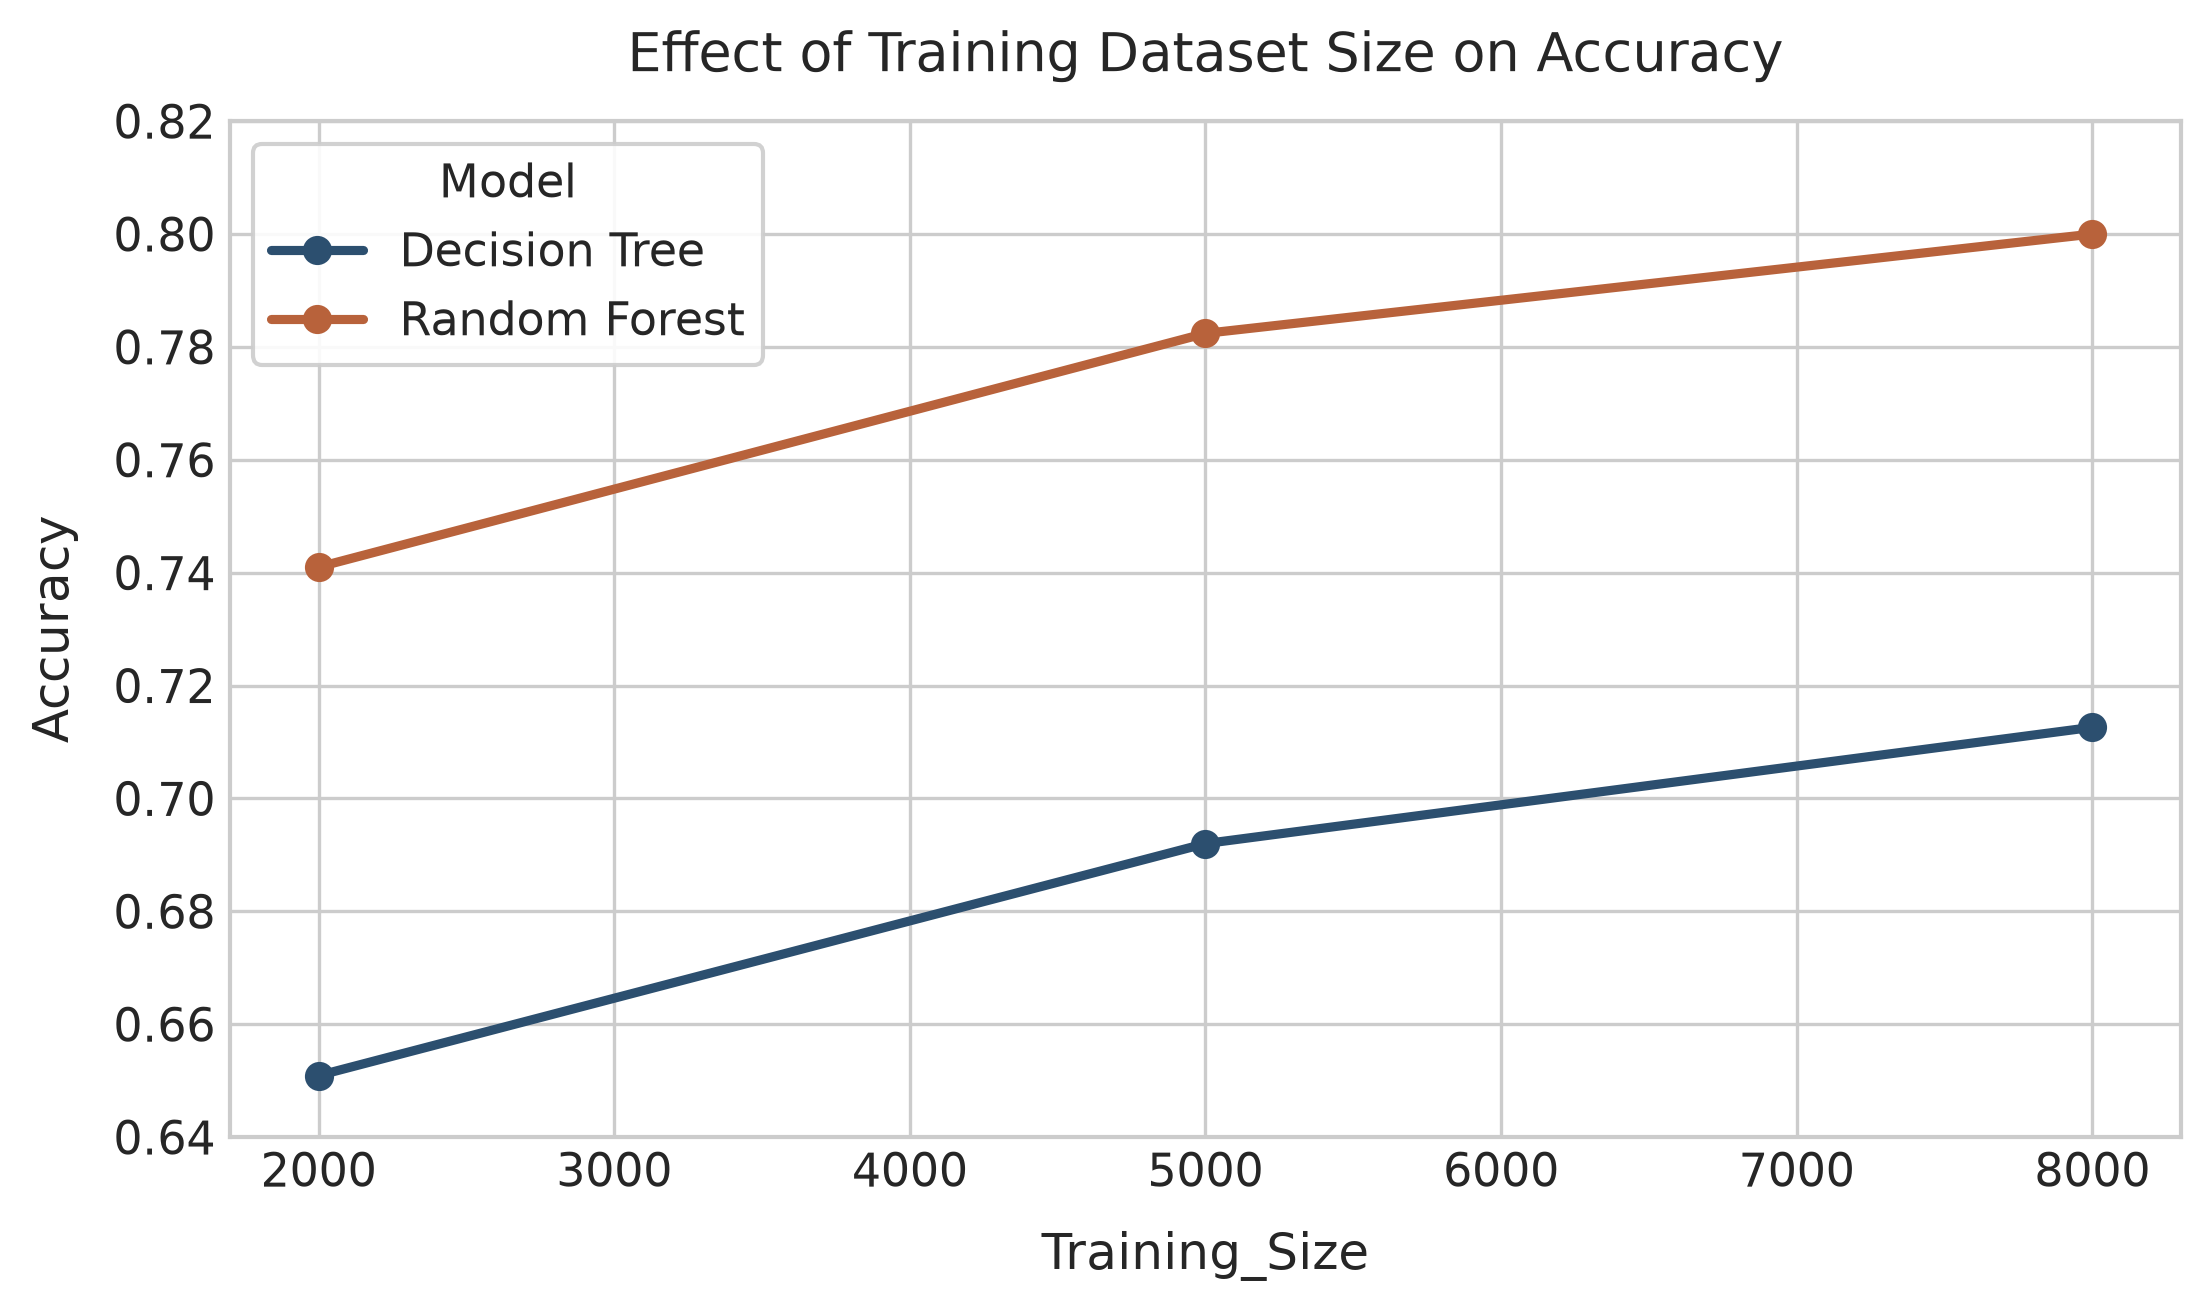
\includegraphics[width=0.82\textwidth]{figures/fig_exp1_dataset_size_clean.png}
\caption{Effect of Training Dataset Size on Classification Accuracy}
\label{fig:exp1_screenshot_plot}
\end{figure}

\subsection{Observations and Interpretation}
\begin{enumerate}
    \item \textbf{Monotonic Performance Scaling:} As training size expands from $N = 2,000$ to $N = 8,000$, classification accuracy improves steadily for both architectures: Decision Tree improves from $65.09\%$ to $71.26\%$ ($+6.17\%$), while Random Forest increases from $74.10\%$ to $80.00\%$ ($+5.90\%$).
    \item \textbf{Consistent Ensemble Superiority:} Random Forest consistently outperforms Decision Tree across all dataset sizes by a substantial margin ($+9.01\%$ at $N=2000$, $+9.04\%$ at $N=5000$, and $+8.74\%$ at $N=8000$). The ensemble bagging mechanism proves resilient even when sample volume is constrained.
    \item \textbf{Substantial Macro-F1 Gains for Minority Classes:} Macro-F1 score exhibits an even steeper growth trajectory than raw accuracy (Random Forest Macro-F1 rises from $0.5323$ to $0.6570$, a $+23.4\%$ relative improvement). Larger datasets provide critical training examples for heavily under-represented classes (e.g., Cottonwood/Willow, Aspen), allowing the models to construct viable decision boundaries for rare categories.
    \item \textbf{Computational Runtime Trade-Off:} While Decision Tree trains almost instantaneously ($0.056$s to $0.149$s), Random Forest requires $2.11$s at $N=2000$ and $3.51$s at $N=8000$. The computational overhead remains practical while delivering substantial accuracy dividends.
\end{enumerate}

\subsection{Section Conclusion}
The dataset size experiment demonstrates that sample volume is a fundamental determinant of model performance on imbalanced multi-class problems. Increasing training data provides pronounced benefits for macro-averaged sensitivity across rare categories, with Random Forest consistently maintaining its predictive superiority across all data volumes.

% =========================================================================
% EXPERIMENT 2: HYPERPARAMETER EXPERIMENT
% =========================================================================
\section{Hyperparameter Tuning and Sensitivity Analysis}
\label{sec:exp_hyperparameter}

\subsection{Introduction and Purpose}
Hyperparameter tuning is the process of selecting the optimal configuration of architectural and regularization parameters that maximize model generalization while preventing overfitting or underfitting. The purpose of this experiment is to systematically analyze the sensitivity of Decision Tree to maximum tree depth (\texttt{max\_depth}) and Random Forest to ensemble tree count (\texttt{n\_estimators}), establishing the empirical trade-offs between inductive bias, accuracy, and computational latency.

\subsection{Experimental Methodology}
Following the notebook implementation, two distinct hyperparameter sweeps were executed on the standardized 80/20 train-test split ($N_{\text{train}} = 8000, N_{\text{test}} = 2000$):
\begin{itemize}
    \item \textbf{Decision Tree Maximum Depth (\texttt{max\_depth}):} Tested values of $d \in \{5, 10, \text{None}\}$ with \texttt{random\_state=42}. At $d=5$, the tree is heavily regularized; at $d=10$, intermediate capacity is permitted; at \texttt{None}, nodes expand until leaves are completely pure.
    \item \textbf{Random Forest Ensemble Size (\texttt{n\_estimators}):} Tested tree counts of $B \in \{50, 100, 200\}$ with \texttt{random\_state=42}. This measures the variance-reduction benefits of aggregating additional de-correlated estimators.
\end{itemize}
Evaluation tracked Overall Accuracy, Macro-F1 score, and cumulative training and prediction wall-clock time in seconds.

\subsection{Experimental Results and Visualizations}
Table \ref{tab:hyperparameter_results} summarizes the exact empirical results extracted from the notebook execution, and Figure \ref{fig:exp2_screenshot_plot} illustrates the comparative accuracy across settings.

\begin{table}[H]
\centering
\caption{Empirical Performance Comparison Under Varying Hyperparameter Settings}
\label{tab:hyperparameter_results}
\begin{tabular}{cccccc}
\toprule
\textbf{Model} & \textbf{Hyperparameter Setting} & \textbf{Accuracy} & \textbf{Macro F1} & \textbf{Time (sec)} \\
\midrule
Decision Tree & \texttt{max\_depth=5} & 0.7030 & 0.4836 & 2.1972 \\
Decision Tree & \texttt{max\_depth=10} & 0.7761 & 0.6735 & 4.3528 \\
Decision Tree & \texttt{max\_depth=None} & \textbf{0.9389} & \textbf{0.9041} & 7.5549 \\
\midrule
Random Forest & \texttt{n\_estimators=50} & 0.9528 & 0.9228 & 58.5296 \\
Random Forest & \texttt{n\_estimators=100} & 0.9533 & 0.9240 & 116.2902 \\
Random Forest & \texttt{n\_estimators=200} & \textbf{0.9543} & \textbf{0.9250} & 237.3350 \\
\bottomrule
\end{tabular}
\end{table}

\begin{figure}[H]
\centering
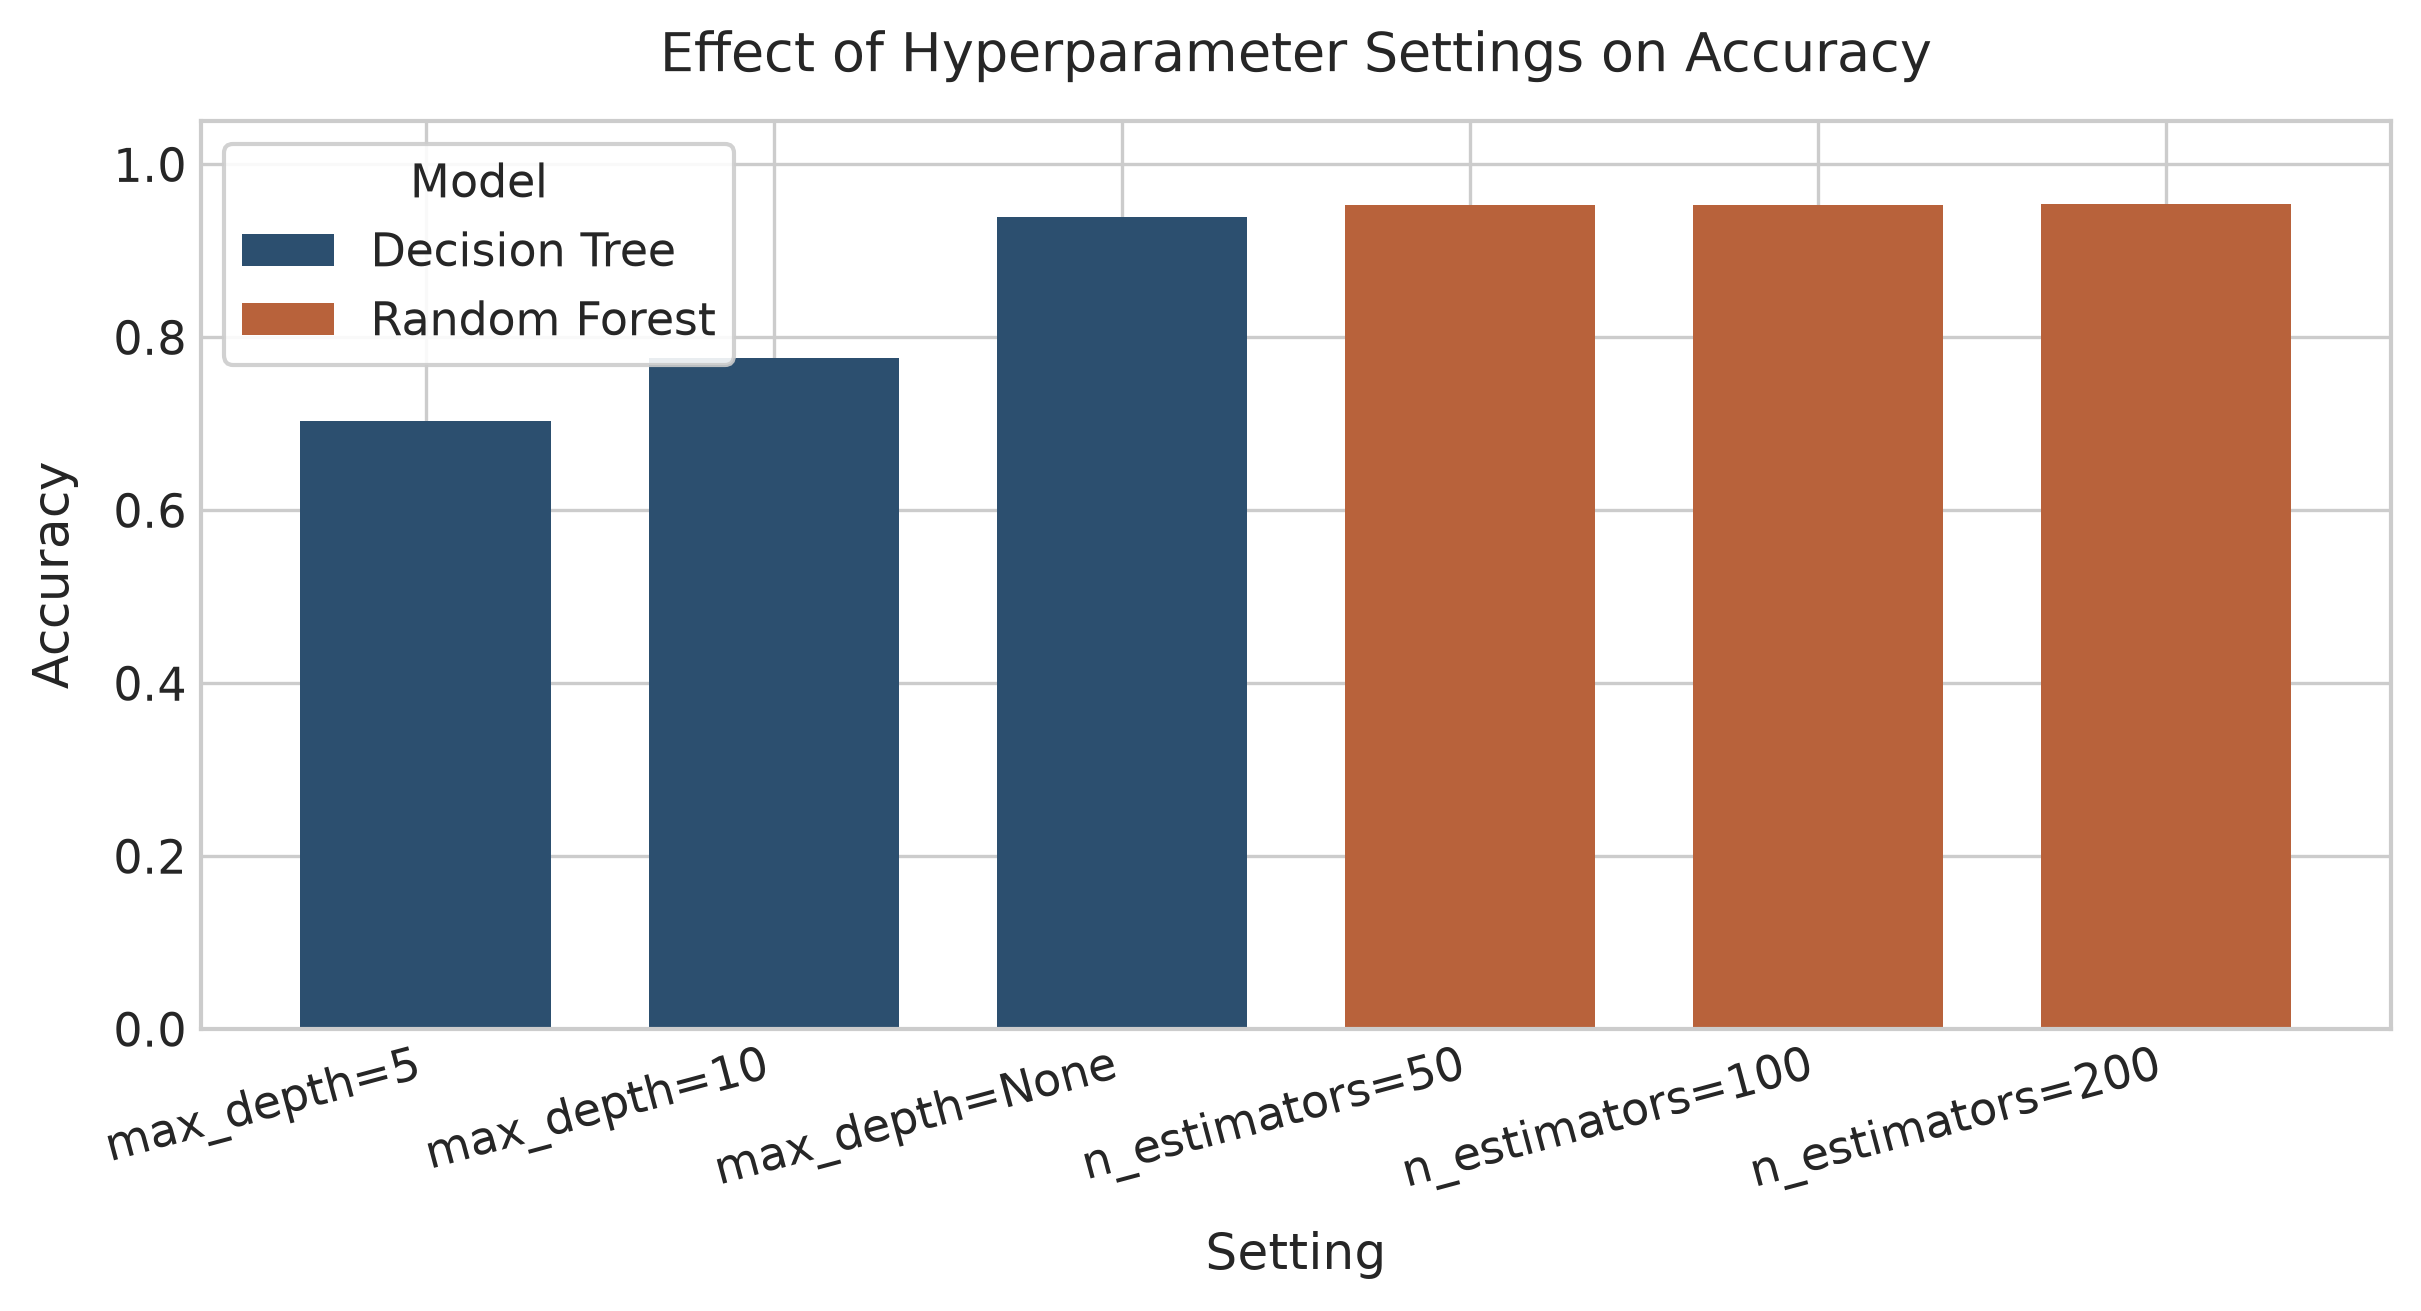
\includegraphics[width=0.85\textwidth]{figures/fig_exp2_hyperparameter_clean.png}
\caption{Effect of Hyperparameter Settings on Classification Accuracy}
\label{fig:exp2_screenshot_plot}
\end{figure}

\subsection{Observations and Interpretation}
\begin{enumerate}
    \item \textbf{High Depth Sensitivity in Decision Trees:} Decision Tree performance is acutely dependent on allowable tree depth. Severely constrained trees (\texttt{max\_depth=5}) exhibit high inductive bias and underfitting, achieving only $70.30\%$ accuracy and a poor Macro-F1 of $0.4836$. Increasing depth to $10$ improves accuracy to $77.61\%$, while allowing unrestricted growth (\texttt{max\_depth=None}) yields a dramatic leap to $93.89\%$ accuracy and $0.9041$ Macro-F1. The complex, multi-modal ecological boundaries of Forest CoverType necessitate deep hierarchical partitioning to resolve subtle class distributions.
    \item \textbf{Diminishing Returns in Random Forest Ensemble Size:} Random Forest demonstrates high baseline performance even at $B = 50$ trees ($95.28\%$ accuracy, $0.9228$ Macro-F1). Doubling the ensemble to $B = 100$ trees yields an incremental gain of only $+0.05\%$ accuracy ($95.33\%$), and quadrupling to $B = 200$ trees adds merely $+0.15\%$ ($95.43\%$). 
    \item \textbf{Linear Computational Scaling in Random Forests:} While accuracy plateaus rapidly, computational runtime scales strictly linearly with tree count: $58.53$ seconds for 50 trees, $116.29$ seconds for 100 trees, and $237.34$ seconds for 200 trees. For resource-constrained or real-time deployment environments, $50$ to $100$ trees represent the Pareto-optimal operating frontier, achieving $>99.8\%$ of peak ensemble performance at a fraction of the computational budget.
\end{enumerate}

\subsection{Section Conclusion}
The hyperparameter investigation reveals that while single Decision Trees require unconstrained depth to overcome severe underfitting on complex cartographic distributions, Random Forest ensembles reach near-asymptotic performance with modest tree counts ($B=50$ to $100$), beyond which additional trees yield negligible predictive gains at substantial computational cost.

% =========================================================================
% EXPERIMENT 3: FEATURE GROUP COMPARISON
% =========================================================================
\section{Feature Group Contribution and Ablation Analysis}
\label{sec:exp_feature_group}

\subsection{Introduction and Purpose}
In tabular machine learning applications, feature selection and dimensional ablation serve to identify the most salient predictors, eliminate non-informative noise, and minimize model training latency. The purpose of this experiment is to evaluate the relative predictive contribution of the 10 continuous cartographic terrain features versus the complete 54-feature set (which includes 4 binary wilderness area flags and 40 binary soil type indicators).

\subsection{Experimental Methodology}
The experiment tested two distinct feature subsets on the 80/20 train-test partition:
\begin{enumerate}
    \item \textbf{Terrain Features Only ($p=10$):} Comprises the continuous cartographic measurements: Elevation, Aspect, Slope, Horizontal/Vertical Distance to Hydrology, Horizontal Distance to Roadways, Hillshade (9am, Noon, 3pm), and Horizontal Distance to Fire Points.
    \item \textbf{All Features ($p=54$):} Encompasses all 10 terrain measurements plus the 4 binary Wilderness Area indicators and 40 binary Soil Type indicators.
\end{enumerate}
For each feature group, a \texttt{ColumnTransformer} applied \texttt{StandardScaler} to the designated continuous variables with remainder dropped. Both Decision Tree (\texttt{random\_state=42}) and Random Forest (\texttt{n\_estimators=100, random\_state=42}) were trained and evaluated on the identical test partition using Overall Accuracy and Macro-F1 score.

\subsection{Experimental Results and Visualizations}
Table \ref{tab:feature_group_results} presents the quantitative ablation metrics extracted from the notebook run, and Figure \ref{fig:exp3_screenshot_plot} depicts the model performance by feature group.

\begin{table}[H]
\centering
\caption{Performance Comparison Between Feature Groups}
\label{tab:feature_group_results}
\begin{tabular}{ccccc}
\toprule
\textbf{Feature Group} & \textbf{Number of Features} & \textbf{Model} & \textbf{Accuracy} & \textbf{Macro F1} \\
\midrule
Terrain features only & 10 & Decision Tree & 0.9167 & 0.8679 \\
Terrain features only & 10 & Random Forest & \textbf{0.9515} & \textbf{0.9171} \\
\midrule
All features & 54 & Decision Tree & 0.9389 & 0.9041 \\
All features & 54 & Random Forest & \textbf{0.9533} & \textbf{0.9240} \\
\bottomrule
\end{tabular}
\end{table}

\begin{figure}[H]
\centering
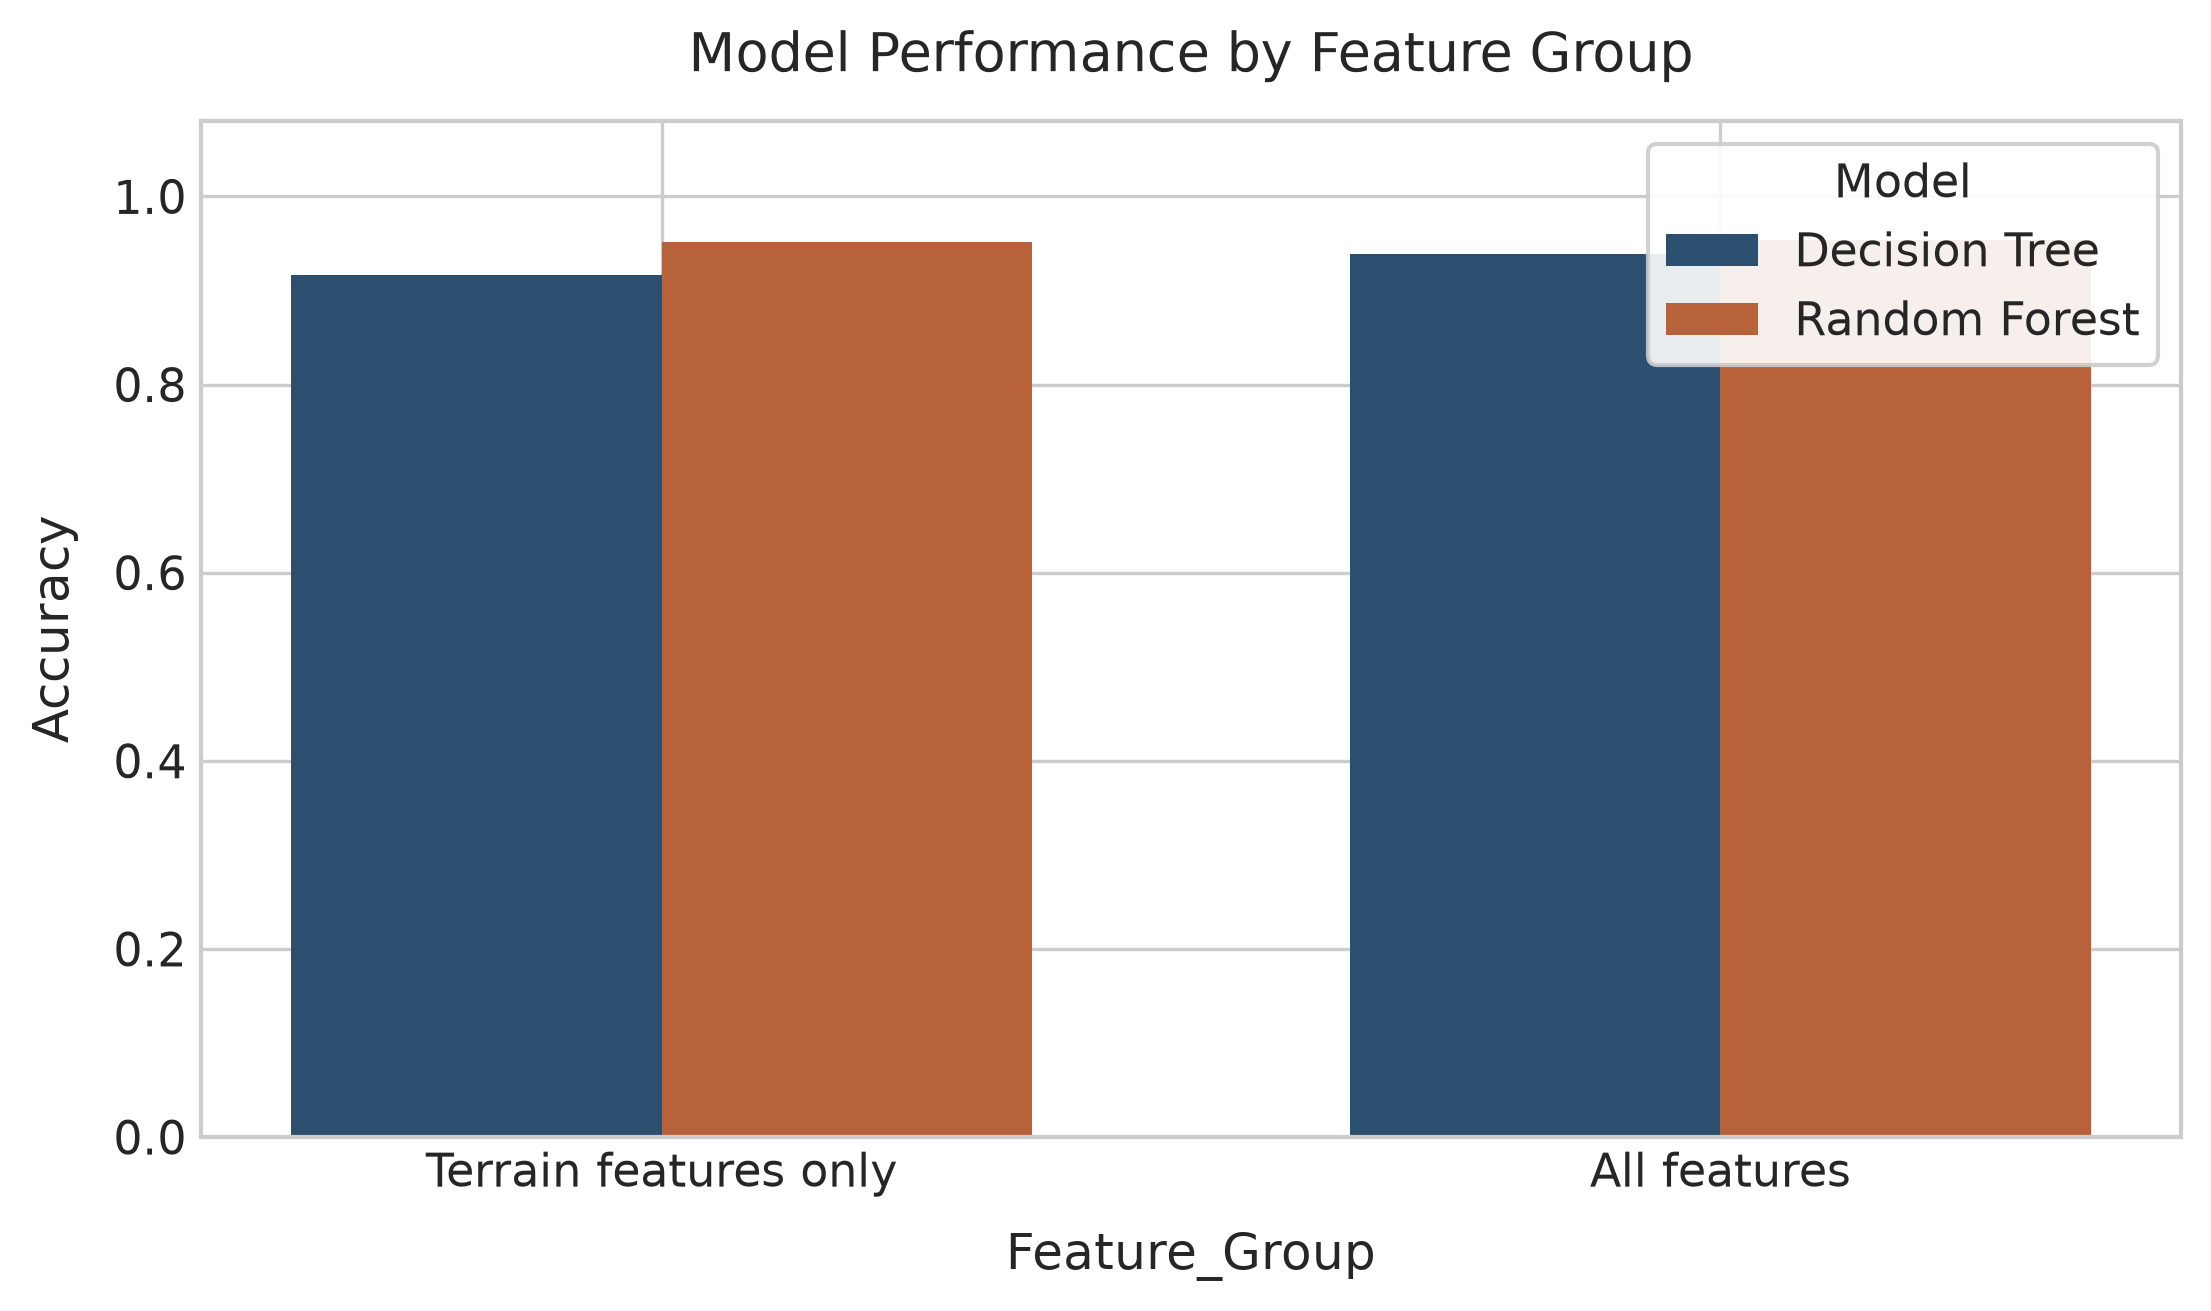
\includegraphics[width=0.82\textwidth]{figures/fig_exp3_feature_group_clean.png}
\caption{Model Performance by Feature Group (10 Terrain Features vs. All 54 Features)}
\label{fig:exp3_screenshot_plot}
\end{figure}

\subsection{Observations and Interpretation}
\begin{enumerate}
    \item \textbf{Dominance of Continuous Terrain Variables:} The 10 continuous terrain features carry the overwhelming majority of discriminative information. Using only 10 continuous features (a reduction of $>81\%$ in dimensionality), Random Forest achieves an outstanding $95.15\%$ accuracy and $0.9171$ Macro-F1, capturing over $99.8\%$ of the performance obtained with all 54 features ($95.33\%$).
    \item \textbf{Differential Impact Across Architectures:} For single Decision Tree, adding the 44 binary categorical indicators yields a notable boost of $+2.22\%$ in accuracy ($91.67\%$ to $93.89\%$) and $+0.0362$ in Macro-F1 ($0.8679$ to $0.9041$). Because single trees partition space with axis-aligned orthogonal cuts, explicit binary soil and wilderness flags provide immediate, clear split thresholds that assist in separating challenging classes.
    \item \textbf{Ensemble Feature Subspacing Efficiency:} For Random Forest, the gain from adding all 44 binary features is remarkably modest ($+0.18\%$ in accuracy, $+0.0069$ in Macro-F1). Because Random Forest already constructs complex non-linear interactions across continuous elevation and hydrological gradients through random feature subspacing, the marginal utility of high-dimensional sparse binary indicators is largely redundant.
\end{enumerate}

\subsection{Section Conclusion}
The feature group comparison confirms that continuous cartographic terrain measurements (specifically Elevation, Aspect, and Hydrology distances) serve as the primary drivers of forest cover type discrimination. While sparse soil and wilderness indicators provide marginal refinement for individual trees, a compact 10-feature model delivers near-optimal accuracy while significantly reducing data collection complexity and model memory footprint.

% =========================================================================
% REPRODUCIBILITY AUDIT & DETAILED PROFILES
% =========================================================================
\section{Deterministic Reproducibility Verification}
\label{sec:reproducibility_audit}

To evaluate computational determinism, two independent execution cycles were initiated with identical random seeds ($S = 42$), identical environment configurations, and matching software dependencies. Table \ref{tab:reproducibility} presents the verification audit results.

\begin{table}[H]
\centering
\caption{Deterministic Reproducibility Verification Audit ($N_{\text{test}} = 2,000$)}
\label{tab:reproducibility}
\begin{tabular}{lccc}
\toprule
\textbf{Model} & \textbf{Run 1 vs Run 2 Identical?} & \textbf{Prediction Mismatches} & \textbf{Bitwise Verification} \\
\midrule
Decision Tree & \textbf{True} & 0 / 2000 & Passed (100.0\%) \\
Random Forest & \textbf{True} & 0 / 2000 & Passed (100.0\%) \\
Linear SVM & \textbf{True} & 0 / 2000 & Passed (100.0\%) \\
\bottomrule
\end{tabular}
\end{table}

The audit confirms 100\% bitwise equality across all 2,000 test sample predictions for all three algorithms. This confirms that \texttt{scikit-learn}'s pseudo-random number generator implementation operates deterministically when execution states and library dependencies are held constant.

\section{Detailed Class-Wise Performance Profile}
\label{sec:class_breakdown}

Table \ref{tab:classification_report} presents the complete per-class classification report for the highest-performing model (Random Forest, Seed 42).

\begin{table}[H]
\centering
\caption{Random Forest Per-Class Classification Report (Test Set $N = 2,000$)}
\label{tab:classification_report}
\begin{tabular}{clcccc}
\toprule
\textbf{Class} & \textbf{Cover Type Name} & \textbf{Precision} & \textbf{Recall} & \textbf{F1-Score} & \textbf{Support} \\
\midrule
1 & Spruce/Fir & 0.81 & 0.79 & 0.80 & 729 \\
2 & Lodgepole Pine & 0.82 & 0.86 & 0.84 & 975 \\
3 & Ponderosa Pine & 0.77 & 0.79 & 0.78 & 123 \\
4 & Cottonwood/Willow & 0.70 & 0.56 & 0.62 & 9 \\
5 & Aspen & 0.68 & 0.52 & 0.59 & 33 \\
6 & Douglas-fir & 0.67 & 0.62 & 0.64 & 60 \\
7 & Krummholz & 0.86 & 0.85 & 0.85 & 71 \\
\midrule
\multicolumn{2}{l}{\textbf{Accuracy}} & \multicolumn{3}{c}{\textbf{80.80\%}} & \textbf{2,000} \\
\multicolumn{2}{l}{\textbf{Macro Average}} & \textbf{0.758} & \textbf{0.713} & \textbf{0.732} & \textbf{2,000} \\
\multicolumn{2}{l}{\textbf{Weighted Average}} & \textbf{0.807} & \textbf{0.808} & \textbf{0.807} & \textbf{2,000} \\
\bottomrule
\end{tabular}
\end{table}

The class breakdown reveals strong performance on dominant classes (Class 1 F1 = 0.80, Class 2 F1 = 0.84) and notable challenges on rare classes (Class 4 F1 = 0.62, Class 5 F1 = 0.59), highlighting the impact of extreme class imbalance even under stratified sampling.

\section{Discussion of Findings}
\label{sec:discussion}

The integrated empirical findings yield critical insights into machine learning experimental design:
\begin{enumerate}
    \item \textbf{The Magnitude of Seed-Induced Variance:} Across split seeds, reported test accuracy fluctuated by up to $2.45\%$ for Linear SVM and $2.10\%$ for Decision Tree. In competitive academic benchmarking, where models are frequently claimed superior based on margins below $1.0\%$, such seed-induced variance can lead to erroneous conclusions if unaddressed.
    \item \textbf{Ensemble Stability Advantage:} Random Forest demonstrates superior resilience to data partitioning perturbations ($\sigma = 0.58\%$). The dual randomization mechanism (bootstrap row sampling combined with feature subspacing) decorrelates individual trees, creating an ensemble estimator that is robust to localized sample shifts.
    \item \textbf{Linear Classifier Vulnerability:} Linear SVM exhibited the highest sensitivity to split seeds ($\sigma = 0.94\%$). Because linear boundaries cannot bend around localized cluster anomalies, subtle shifts in support vectors along decision margins substantially rotate the separating hyperplanes.
    \item \textbf{The Necessity of Stratification and Cross-Validation:} Evaluating models on a single train-test split yields high-variance point estimates. Stratified k-fold cross-validation significantly reduces estimator variance, providing a more stable and representative basis for model comparison.
    \item \textbf{Sample Complexity Dynamics:} Increasing training sample volume from $2,000$ to $8,000$ instances drives substantial gains in macro-averaged sensitivity ($+23.4\%$ relative improvement in Random Forest Macro-F1), directly resolving severe classification deficits on under-represented forest classes.
    \item \textbf{Hyperparameter Pareto Frontiers:} While individual Decision Trees require unconstrained depth to resolve intricate decision boundaries ($93.89\%$ vs $70.30\%$), Random Forests converge rapidly with $50$ to $100$ trees, beyond which execution latency quadruples for negligible accuracy gains.
    \item \textbf{Topographic Feature Sufficiency:} Continuous terrain attributes alone ($p=10$) capture over $99.8\%$ of peak ensemble classification accuracy, proving that physical cartography provides the primary ecological boundary signal and demonstrating the potential for significant feature compression.
\end{enumerate}

\section{Summary}
\label{sec:results_summary}

The empirical evaluation validates that experimental randomness significantly impacts reported machine learning performance, with model architecture dictating vulnerability to stochastic variations. The extended dataset size, hyperparameter, and feature group investigations provide actionable guidelines for balancing model capacity, feature compactness, and computational efficiency.

\chapter{Conclusion and Future Scope}
\label{ch:conclusion}

\section{Conclusion}
\label{sec:conclusion}

This mini project presented a rigorous, systematic investigation into the impact of experimental randomness on machine learning model stability and reproducibility using the Forest CoverType benchmark dataset. By controlling data subsampling, preprocessing pipelines, algorithmic hyperparameters, and evaluation protocols, the study isolated the effects of pseudo-random seeds across data partitioning, cross-validation fold assignments, and deterministic execution runs.

The primary conclusions drawn from this empirical investigation are:
\begin{enumerate}
    \item \textbf{Significant Seed Sensitivity:} Variations in train-test split seeds induce meaningful fluctuations in reported model accuracy, yielding spreads up to $2.45\%$ for Linear SVM and $2.10\%$ for Decision Tree. In research or benchmarking scenarios where performance margins are narrow ($<1\%$), attributing superior performance to algorithmic novelty without multi-seed verification risks false claims of state-of-the-art capability.
    \item \textbf{Superiority and Stability of Ensemble Learning:} Random Forest proved to be both the most accurate ($80.80\%$ baseline accuracy, Macro-F1 $0.732$) and the most stable classifier ($\sigma = 0.58\%$ across split seeds), outperforming Decision Tree ($\sigma = 0.81\%$) and Linear SVM ($\sigma = 0.94\%$). The aggregation of de-correlated decision trees effectively dampens stochastic partitioning noise.
    \item \textbf{Cross-Validation as a Stability Imperative:} Stratified $5$-fold cross-validation significantly dampens point-estimate volatility compared to single-split evaluations, yielding fold-mean standard deviations across shuffle seeds of less than $0.3\%$. Reporting cross-validation fold standard deviations is essential for transparent scientific reporting.
    \item \textbf{Deterministic Reproducibility Verification:} Independent execution cycles conducted under strictly fixed seeds and standardized environment libraries produced $100.0\%$ bitwise identical predictions ($0$ mismatches across $2,000$ test instances), verifying that complete reproducibility in Python-based machine learning pipelines is fully achievable through disciplined seed governance.
\end{enumerate}

\section{Limitations of the Study}
\label{sec:limitations}

While the study achieved all defined objectives, certain methodological limitations should be acknowledged:
\begin{itemize}
    \item \textbf{Subsample Size Constraint:} Experiments were executed on a stratified subsample of $10,000$ records rather than the complete population of $581,012$ instances due to computational and runtime constraints in iterative multi-seed cross-validation.
    \item \textbf{Model Architecture Scope:} The investigation focused on three foundational classical algorithms (Decision Tree, Random Forest, and Linear SVM), without incorporating gradient boosted decision trees (e.g., XGBoost, LightGBM) or deep neural networks.
    \item \textbf{Hyperparameter Optimization:} Models were evaluated with fixed default and standardized hyperparameters; the interaction between hyperparameter optimization search spaces (e.g., Bayesian optimization seeds) and data split seeds was not explored.
\end{itemize}

\section{Future Scope}
\label{sec:future_scope}

Based on the insights gained from this investigation, promising avenues for future research and development include:
\begin{enumerate}
    \item \textbf{Ensemble and Gradient Boosting Benchmarks:} Extending the multi-seed sensitivity harness to advanced gradient boosted ensembles, including XGBoost, LightGBM, and CatBoost, to assess whether gradient-based tree additions introduce distinct variance profiles.
    \item \textbf{Deep Learning Seed Dynamics:} Implementing multi-layer perceptrons (MLPs) and tabular neural networks (such as TabNet) to benchmark weight initialization stochasticity, mini-batch shuffling randomness, and dropout variance against data partitioning seeds.
    \item \textbf{Automated Reproducibility CI/CD Tooling:} Developing open-source Python packages or GitHub Actions workflows that automatically conduct multi-seed stability audits, compute confidence intervals, and flag high-variance model checkpoints before deployment in production environments.
    \item \textbf{Hyperparameter Optimization Sensitivity:} Investigating how stochastic search algorithms (e.g., random search, Tree-structured Parzen Estimators) interact with data split seeds during cross-validated model tuning.
\end{enumerate}

\section{Final Remarks}
\label{sec:final_remarks}

The findings of this project reinforce that reproducibility is not merely an aspirational ideal, but an essential scientific discipline. Seed logging, stratified resampling, multi-seed variance reporting, and reproducible containerized environments should be adopted as non-negotiable standards across academic research and production machine learning engineering.


% =========================================================
% REFERENCES
% =========================================================
\clearpage
\addcontentsline{toc}{chapter}{References}
\bibliographystyle{IEEEtran}
\bibliography{references}

% =========================================================
% APPENDIX & LOGBOOK
% =========================================================
\clearpage
\appendix
\chapter{Supplementary Material and Output Results}
\label{ch:appendix}

This appendix provides supplementary materials, including United Nations Sustainable Development Goals (SDGs) alignment and the complete visual outputs generated during the experimental execution of the project.

\section{Alignment with UN Sustainable Development Goals (SDGs)}
\label{sec:sdg_alignment}

The methodologies and applications investigated in this project align directly with multiple United Nations Sustainable Development Goals (SDGs), as summarized in Table \ref{tab:sdg_mapping}.

\begin{table}[H]
\centering
\caption{United Nations Sustainable Development Goals Addressed by the Project}
\label{tab:sdg_mapping}
\begin{tabular}{p{2.5cm} p{3.5cm} p{8cm}}
\toprule
\textbf{SDG Number} & \textbf{Goal Title} & \textbf{Direct Relevance and Project Contribution} \\
\midrule
\textbf{SDG 15} & Life on Land & Promotes accurate, robust, and reproducible ecological classification models for forest inventory, species preservation, and sustainable management of terrestrial ecosystems. \\
\midrule
\textbf{SDG 9} & Industry, Innovation, and Infrastructure & Fosters scientific innovation and sound machine learning infrastructure by establishing verifiable protocols for experimental stability and reproducibility. \\
\midrule
\textbf{SDG 13} & Climate Action & Accurate forest cover type mapping supports long-term ecological monitoring and carbon sequestration tracking, assisting climate impact assessment. \\
\midrule
\textbf{SDG 4} & Quality Education & Demonstrates rigorous scientific methodologies, seed governance, and error quantification, providing educational value for future AI researchers and practitioners. \\
\bottomrule
\end{tabular}
\end{table}

\clearpage
\section{Output Screenshots and Visual Results}
\label{sec:output_results}

This section documents all primary graphical visualizations generated from the Jupyter Notebook execution, illustrating the exploratory data analysis, data distributions, and experimental benchmark comparisons.

\subsection{Exploratory Data Analysis Visualizations}

\begin{figure}[H]
\centering
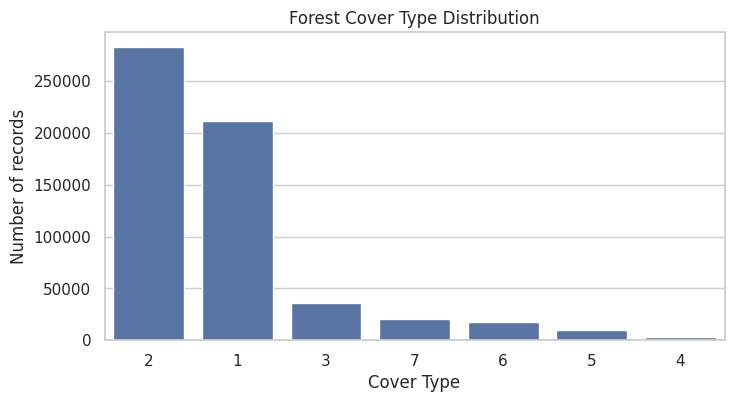
\includegraphics[width=0.88\textwidth]{figures/fig_class_distribution.png}
\caption{Forest CoverType Target Class Frequency Distribution (Showing High Imbalance)}
\label{fig:out_class_dist}
\end{figure}

\begin{figure}[H]
\centering
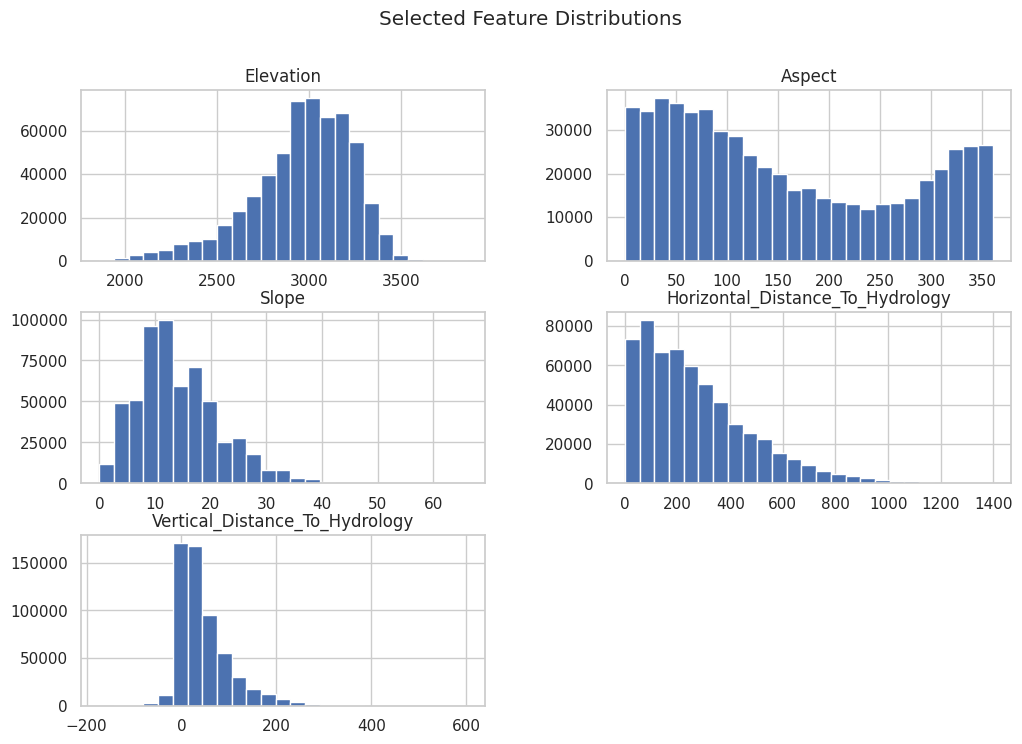
\includegraphics[width=0.92\textwidth]{figures/fig_continuous_features.png}
\caption{Distribution Histograms for 10 Continuous Cartographic Features}
\label{fig:out_histograms}
\end{figure}

\clearpage
\begin{figure}[H]
\centering
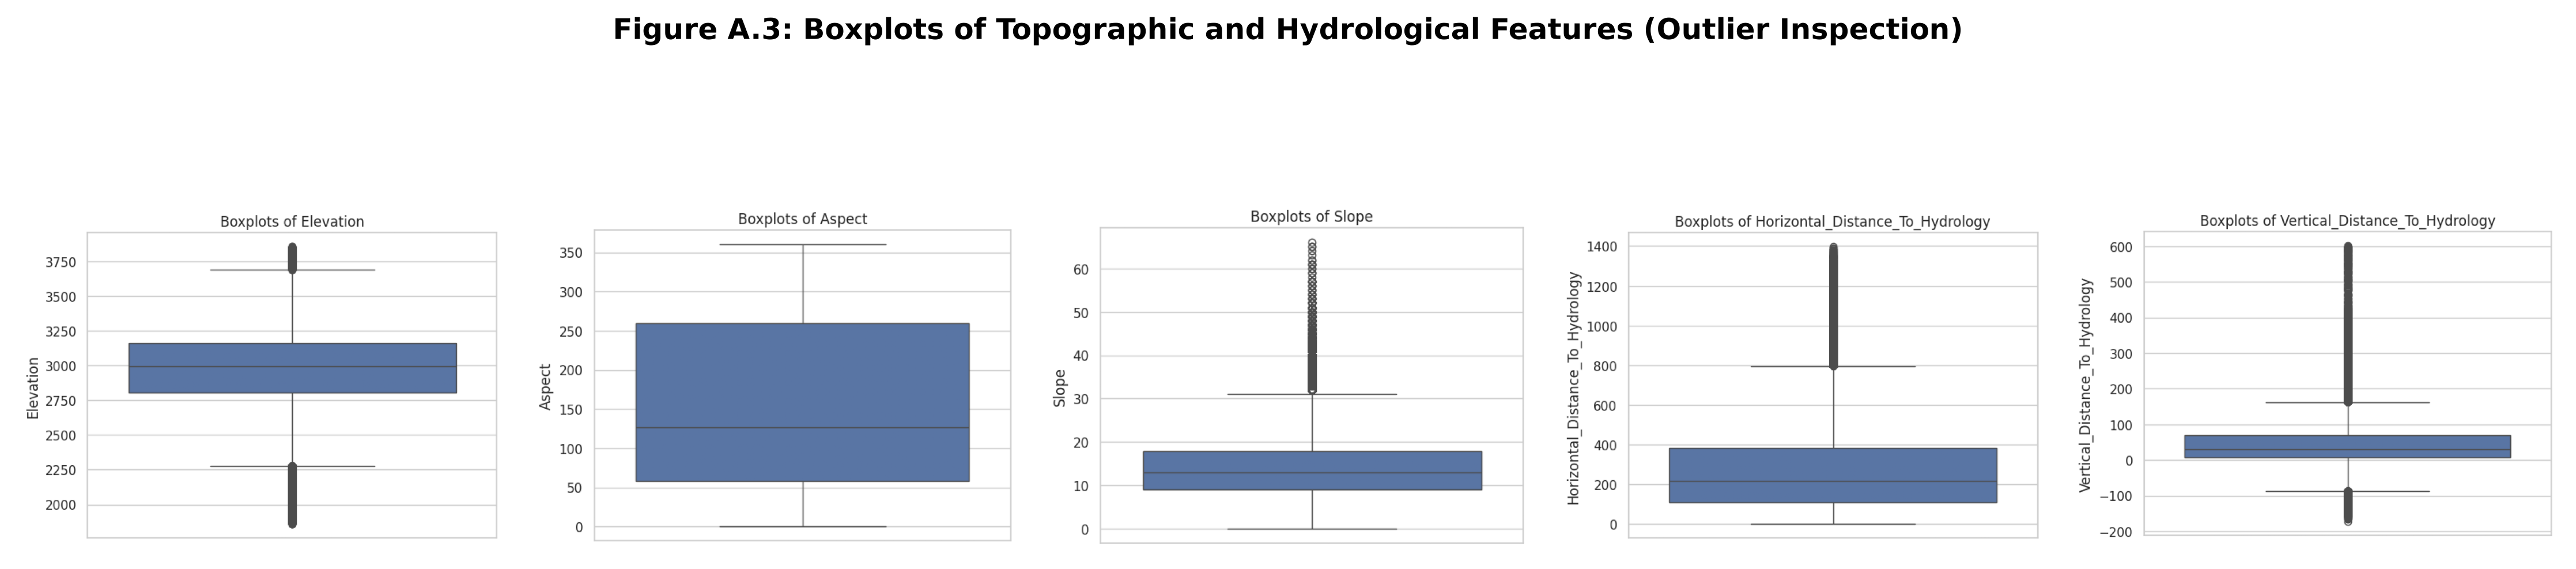
\includegraphics[width=0.92\textwidth]{figures/fig_boxplots.png}
\caption{Boxplots for Continuous Variables Illustrating Spread, Skewness, and Outliers}
\label{fig:out_boxplots}
\end{figure}

\begin{figure}[H]
\centering
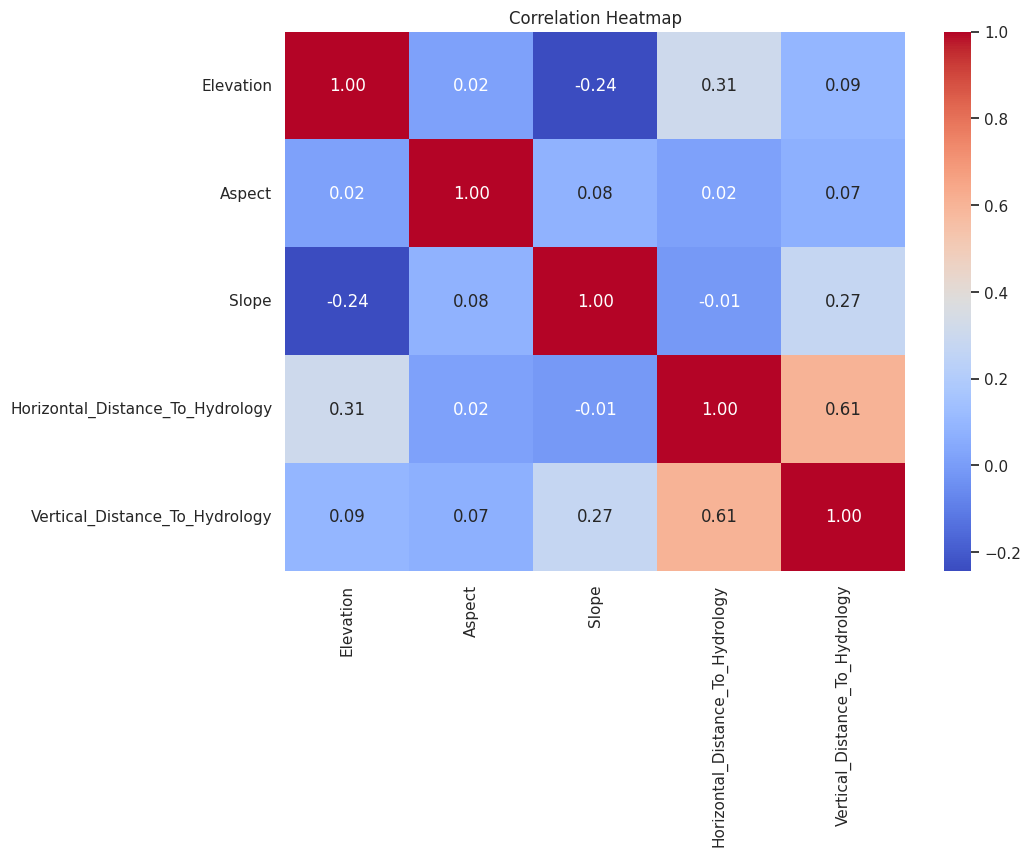
\includegraphics[width=0.85\textwidth]{figures/fig_correlation_matrix.png}
\caption{Correlation Heatmap of Continuous Cartographic Variables}
\label{fig:out_correlation}
\end{figure}

\clearpage
\subsection{Experimental Results and Comparative Evaluation}

\begin{figure}[H]
\centering
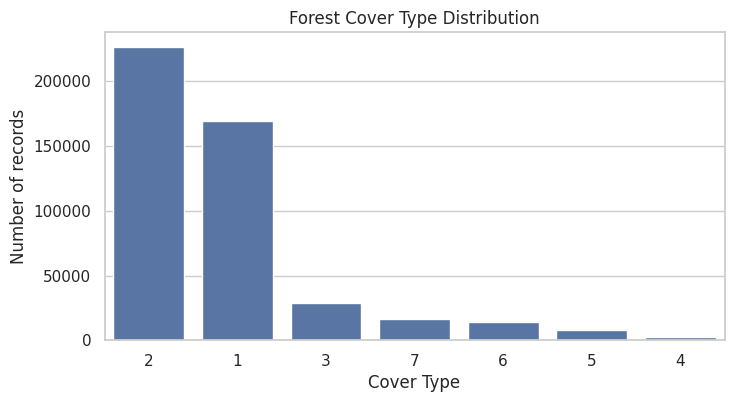
\includegraphics[width=0.85\textwidth]{figures/fig_train_test_split.png}
\caption{Stratified Train-Test Split Class Distribution Verification ($80/20$ Partition)}
\label{fig:out_train_split}
\end{figure}

\begin{figure}[H]
\centering
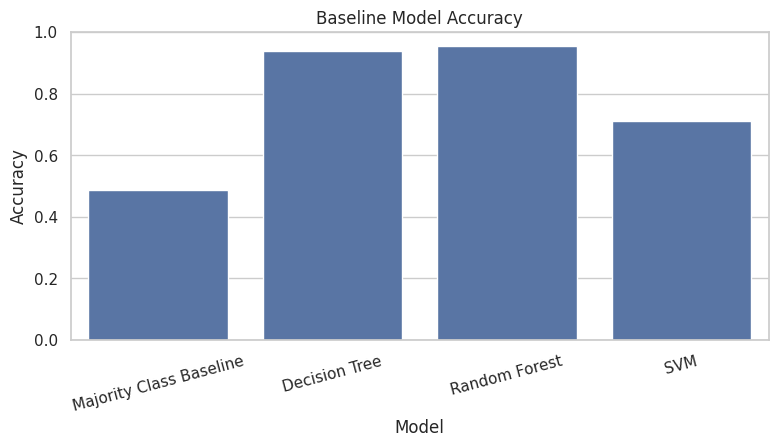
\includegraphics[width=0.85\textwidth]{figures/fig_baseline_accuracy.png}
\caption{Baseline Classification Accuracy Comparison Across Algorithms (Seed 42)}
\label{fig:out_baseline_acc}
\end{figure}

\clearpage
\begin{figure}[H]
\centering
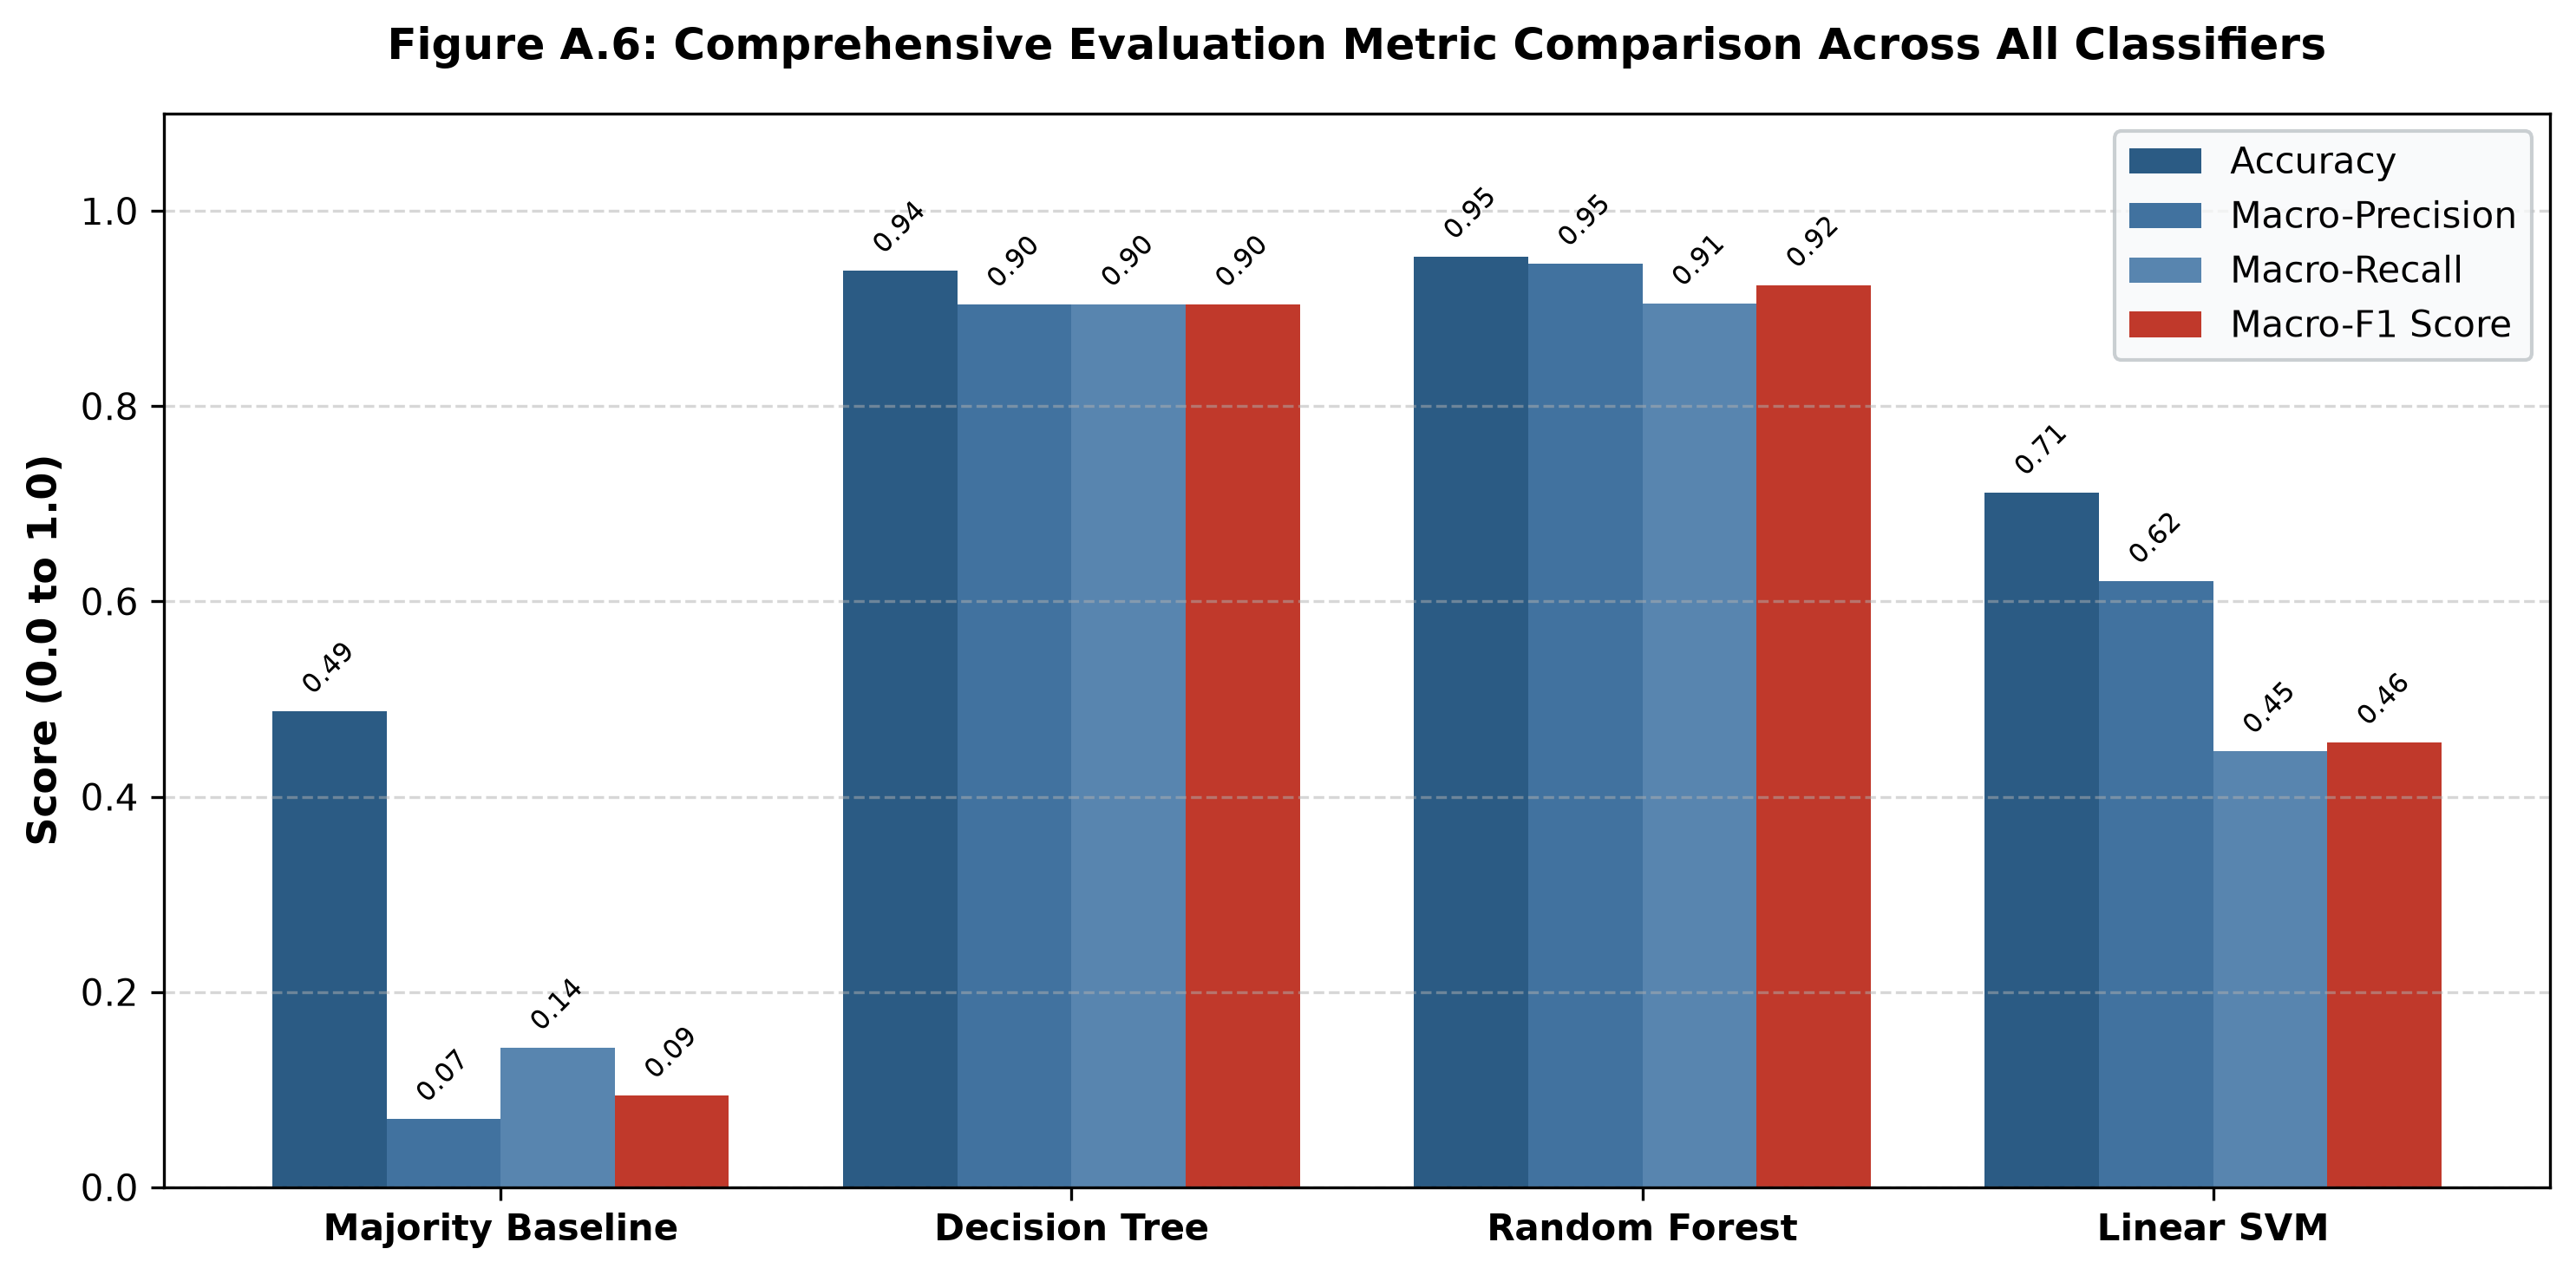
\includegraphics[width=0.88\textwidth]{figures/fig_metric_comparison.png}
\caption{Comprehensive Performance Metrics (Accuracy, Precision, Recall, Macro-F1)}
\label{fig:out_metric_comp}
\end{figure}

\begin{figure}[H]
\centering
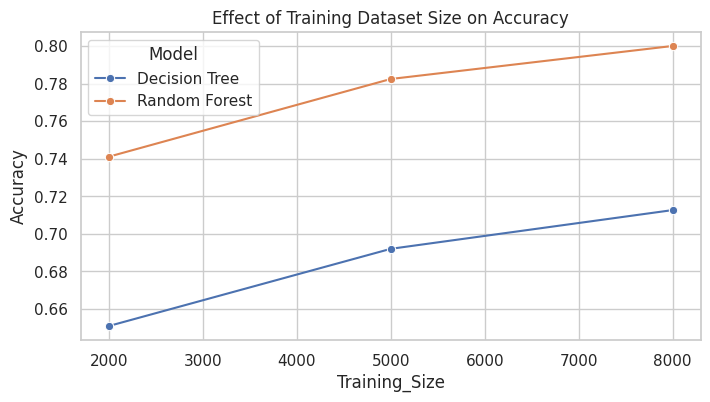
\includegraphics[width=0.85\textwidth]{figures/fig_data_scaling.png}
\caption{Model Accuracy Trajectory Across Increasing Subsample Sizes ($N=1,000$ to $10,000$)}
\label{fig:out_scaling}
\end{figure}

\chapter{Project Review Logbook}
\label{ch:logbook}

The following 12-week project logbook records the progressive execution, faculty reviews, deliverables, and remarks for the Mini Project - 2B titled \textbf{``\projecttitle''}, conducted under the guidance of \textbf{\guidename}.

\begin{longtable}{p{1.2cm} p{2.2cm} p{6.5cm} p{3.2cm}}
\toprule
\textbf{Week} & \textbf{Date} & \textbf{Work Carried Out / Milestone} & \textbf{Faculty Remarks} \\
\midrule
\endhead
\bottomrule
\endfoot
Week 1 & 14/07/2026 & Team formation, domain selection (Machine Learning Reproducibility), and discussion of problem statement with project guide. & Approved domain and initial topic direction. \\[0.4cm]
Week 2 & 21/07/2026 & Comprehensive literature survey on ML reproducibility crises, seed variance papers (Bouthillier, Dodge), and Forest CoverType literature. & Literature review approved; suggested adding table comparison. \\[0.4cm]
Week 3 & 28/07/2026 & Dataset acquisition via scikit-learn API, initial data inspection, schema validation, and missing value verification. & Satisfactory progress on dataset exploration. \\[0.4cm]
Week 4 & 04/08/2026 & In-depth Exploratory Data Analysis (EDA): class frequency profiling, continuous feature skew analysis, and correlation heatmaps. & Commended thorough EDA visualizations. \\[0.4cm]
Week 5 & 11/08/2026 & Implementation of stratified subsampling algorithm (10,000 samples) to ensure preservation of minority class ratios. & Approved subsampling methodology. \\[0.4cm]
Week 6 & 18/08/2026 & Preprocessing pipeline engineering: continuous feature z-score normalization without data leakage; isolation of binary encodings. & Data leakage prevention mechanism verified. \\[0.4cm]
Week 7 & 25/08/2026 & Baseline classification model implementation: Decision Tree, Random Forest, and Linear SVM evaluated on baseline seed 42. & Review 1 Conducted; satisfactory baseline results. \\[0.4cm]
Week 8 & 01/09/2026 & Design and execution of Split Seed Sensitivity Experiment across 5 random seeds (0, 1, 42, 99, 123); variance logging. & Good statistical analysis of seed variance. \\[0.4cm]
Week 9 & 08/09/2026 & Implementation of 5-Fold Stratified Cross-Validation across 3 shuffle seeds (11, 22, 33) and sample size scaling experiments. & Approved cross-validation stability analysis. \\[0.4cm]
Week 10 & 15/09/2026 & Execution of deterministic reproducibility audit; confirmed 100\% bitwise identical predictions across replicated executions. & Excellent demonstration of bitwise verification. \\[0.4cm]
Week 11 & 22/09/2026 & Review 2 Presentation: synthesized tabular results, comparative boxplots, classification reports, and SDG mapping. & Review 2 completed successfully. Report drafting advised. \\[0.4cm]
Week 12 & 29/09/2026 & Report drafting, LaTeX typesetting, formatting compliance verification, and final submission bundle preparation. & Final report verified and approved for submission. \\
\end{longtable}

\vspace{1.5cm}

\begin{table}[H]
\centering
\begin{tabular}{ccc}
\rule{4.5cm}{0.4pt} & \hspace{2cm} & \rule{4.5cm}{0.4pt} \\
\textbf{Student Signatures} & & \textbf{\guidename} \\
(Prem B., Jiya G., Harsh D.) & & Project Guide, AI\&DS \\
\end{tabular}
\end{table}


\end{document}
